\documentclass[hidelinks, a4paper, 12pt, oneside]{report}         %% LaTeX2e document.
\usepackage {tcdthesis}              %% Preamble.
\usepackage{graphicx,color, colortbl}
\usepackage{anysize}
\usepackage{amsmath}
\usepackage{hyperref}
\usepackage{array}
\usepackage{listings}
\usepackage{longtable}
\newcolumntype{L}[1]{>{\raggedright\let\newline\\\arraybackslash\hspace{0pt}}m{#1}}
\newcolumntype{C}[1]{>{\centering\let\newline\\\arraybackslash\hspace{0pt}}m{#1}}
\newcolumntype{R}[1]{>{\raggedleft\let\newline\\\arraybackslash\hspace{0pt}}m{#1}}

\mastersthesis                     %% Uncomment one of these; if you don't
%\phdthesis                         %% use either, the default is \phdthesis.

%\thesisdraft                       %% Uncomment this if you want a draft
                                     %% version; this will print a timestamp
                                     %% on each page of your thesis.

\leftchapter                       %% Uncomment one of these if you want
%\centerchapter                      %% left-justified, centered or
% \rightchapter                      %% right-justified chapter headings.
                                     %% Chapter headings includes the
                                     %% Contents, Acknowledgments, Lists
                                     %% of Tables and Figures and the Vita.
                                     %% The default is \centerchapter.

% \singlespace                       %% Uncomment one of these if you want
% \oneandhalfspace                   %% single-spacing, space-and-a-half
 \doublespace                       %% or double-spacing; the default is
                                     %% \oneandhalfspace, which is the
                                     %% minimum spacing accepted by the
                                     %% Graduate School.

\renewcommand{\thesisauthor}{Harpreet Singh}            %% Your official UT name.
\renewcommand{\thesismonth}{September}                  %% Your month of graduation.
\renewcommand{\thesisyear}{2016}                      %% Your year of graduation.
\renewcommand{\thesistitle}{\large{} \\ \LARGE{Proactive Configuration of Data Centre Networks for Big Data Processing}}            %% The title of your thesis; use mixed-case.
\renewcommand{\thesisauthorpreviousdegrees}{B.Sc.}  %% Your previous degrees, abbreviated; separate multiple degrees by commas.
\renewcommand{\thesissupervisor}{Stefan Weber}      %% Your thesis supervisor; use mixed-case and don't use any titles or degrees.

% \renewcommand{\thesiscosupervisor}{}                 %% Your PhD. thesis co-supervisor; if any.

\renewcommand{\thesisauthoraddress}{Dublin, Ireland}

%\renewcommand{\thesisdedication}{...}     %% Your dedication, if you have one; use "\\" for linebreaks.


%%%%%%%%%%%%%%%%%%%%%%%%%%%%%%%%%%%%%%%%%%%%%%%%%%%%%%%%%%%%%%%%%%%%%%%%%%%%%
%%%
%%% The following commands are all optional, but useful if your requirements
%%% are different from the default values in utthesis.sty.  To use them,
%%% simply uncomment (remove the leading %) the line(s).

% \renewcommand{\thesiscommitteesize}{...}
                                     %% Uncomment this only if your thesis
                                     %% committee does NOT have 5 members
                                     %% for \phdthesis or 2 for \mastersthesis.
                                     %% Replace the "..." with the correct
                                     %% number of members.

\renewcommand{\thesisdegree}{Master of Science in Computer Science}  %% Uncomment this only if your thesis
                                     %% degree is NOT "DOCTOR OF PHILOSOPHY"
                                     %% for \phdthesis or "MASTER OF ARTS"
                                     %% for \mastersthesis.  Provide the
                                     %% correct FULL OFFICIAL name of
                                     %% the degree.

\renewcommand{\thesisdegreeabbreviation}{M.Sc.}
                                     %% Use this if you also use the above
                                     %% command; provide the OFFICIAL
                                     %% abbreviation of your thesis degree.

\renewcommand{\thesistype}{Dissertation}    %% Use this ONLY if your thesis type
                                     %% is NOT "Dissertation" for \phdthesis
                                     %% or "Thesis" for \mastersthesis.
                                     %% Provide the OFFICIAL type of the
                                     %% thesis; use mixed-case.
%%%
%%%%%%%%%%%%%%%%%%%%%%%%%%%%%%%%%%%%%%%%%%%%%%%%%%%%%%%%%%%%%%%%%%%%%%%%%%%%%

%%%%
%%%% Commands for highlighting JSON snippet
%%%%
\newcommand\JSONnumbervaluestyle{\color{blue}}
\newcommand\JSONstringvaluestyle{\color{red}}

% switch used as state variable
\newif\ifcolonfoundonthisline

\makeatletter

\lstdefinestyle{json}
{
	showstringspaces    = false,
	keywords            = {false,true},
	alsoletter          = 0123456789.,
	morestring          = [s]{"}{"},
	stringstyle         = \ifcolonfoundonthisline\JSONstringvaluestyle\fi,
	MoreSelectCharTable =%
	\lst@DefSaveDef{`:}\colon@json{\processColon@json},
	basicstyle          = \linespread{0.9}\ttfamily,
	keywordstyle        = \ttfamily\bfseries,
}
% flip the switch if a colon is found in Pmode
\newcommand\processColon@json{%
	\colon@json%
	\ifnum\lst@mode=\lst@Pmode%
	\global\colonfoundonthislinetrue%
	\fi
}

\lst@AddToHook{Output}{%
	\ifcolonfoundonthisline%
	\ifnum\lst@mode=\lst@Pmode%
	\def\lst@thestyle{\JSONnumbervaluestyle}%
	\fi
	\fi
	%override by keyword style if a keyword is detected!
	\lsthk@DetectKeywords% 
}

% reset the switch at the end of line
\lst@AddToHook{EOL}%
{\global\colonfoundonthislinefalse}

\makeatother

%%%%%%%%%%%%%%%%%%%%%%%%%%%%%%%%%%%%%%%%%%%%%%%


\begin{document}                                  %% BEGIN THE DOCUMENT


\thesistitlepage                                  %% Generate the title page.

\thesisdeclarationpage				  %% Generate the declaration page.

\thesispermissionpage				  %% Generate the copyright permission page

%\thesisdedicationpage                             %% Generate the dedication page.

\begin{thesisacknowledgments}                     %% Use this to write your
			                          %% acknowledgements; it can be anything
Firstly, I would like to thank my supervisor Stefan Weber for making this dissertation possible with his invaluable guidance and support. I would also like to thank my family and friends, for their encouragement. And finally, I would like to thank Alexia, for her infallible moral support and encouragement.  

\end{thesisacknowledgments}                       %% allowed in LaTeX2e par-mode.

\begin{thesisabstract}

Various studies have determined that the network is a performance \textit{bottleneck} in Big Data processing applications running in the cloud such as Hadoop. Numerous attempts have been made to alleviate this network bottleneck by traffic engineering during execution of the applications, using Software-Defined Networking. Such measures of traffic engineering are overwhelmingly \textit{reactive} in nature and are bound to induce control traffic overhead in the network. In this project, we propose a \textit{proactive} approach for configuring Data Centre Networks as the means to optimize application traffic, specifically Hadoop; thereby accelerating the execution of applications in the cloud. 

    We configure the network before execution of the application, to determine if there is a performance gain when there is no control overhead in the network. The network is configured \textit{proactively}, by logging the flow decisions made by the \textit{reactive} algorithms from previous studies. These flow rules are subsequently installed in the routing devices before the execution of the application, after which, the flows are routed \textit{reactively}. We demonstrate an \textit{average gain in network bandwidth utilization} between 11.9\% to 59.9\% in comparison to \textit{reactive} approaches, while Hadoop job completion times are reduced by 10\% to 33.5\%.         

\end{thesisabstract}

\tableofcontents                                  %% Generate table of contents.
\listoftables                                     %% Uncomment this to generate list of tables.
\listoffigures                                    %% Uncomment this to generate list of figures.

%%
%% Include thesis chapters here...
%%
  \chapter{Introduction}


The ever growing organisations involved in search engines, social networking as well as applications for mobile devices, require efficient analysis of the massive collections of the data generated, which is achieved using thousands of commodity servers, resulting in the growing trend of \textit{Big Data Analytics} \cite{mcafee2012big}. Big data applications process data by distributing it across the data centre clusters, and after each piece has been analysed in parallel, the final data set is transferred and merged across the data centre network.

To support such communication patterns, data centre topologies make use of \textit{multi-rooted tree} topologies in order to achieve higher speed links among the clusters and bypass the limitations caused by \textit{limited port densities} in commodity switches \cite{al2010hedera}. The goal of \textit{multi-rooted tree} topologies is to enable efficient communication among the network hosts by increasing the number of paths that interconnect them, thereby creating redundancy. Path multiplicity in \textit{multi-rooted tree topologies} is achieved by horizontal scaling of hosts \cite{al2008scalable, greenberg2009vl2, guo2008dcell,guo2009bcube} in order to cater to the increasing processing demands of big data applications.

Traditional network traffic routing protocols are designed for much simplistic communication patterns and topologies, with limited paths between host destination pairs, where the small number of redundant paths are used for fault tolerance, making them not suitable to be used for routing traffic in topologies with path diversity. Additional obstacles in routing of big data application traffic are possible escalation in network traffic volumes, multiplicity of traffic patterns and high duration of data processing jobs. As a result, various studies \cite{al2010hedera, greenberg2009vl2,guo2008dcell} have highlighted that the network is a bottleneck in the performance of big data applications. 

A significant amount of research \cite{das2013transparent, wang2012programming, al2010hedera, narayan2012hadoop, neves2014pythia, wette2015hybridte} has been conducted with the sole purpose of optimizing traffic in a data centre network for large-scale data analysis by devising new flow scheduling mechanisms and programming the entire network stack, so as to maximize throughput in the network, enabling better performance of big data applications. All work done in this field employs the emergent technology of Software-Defined Networking (SDN), in order to configure the network in accordance with big data application communication patterns.  

\begin{figure}[!ht]
\centerline{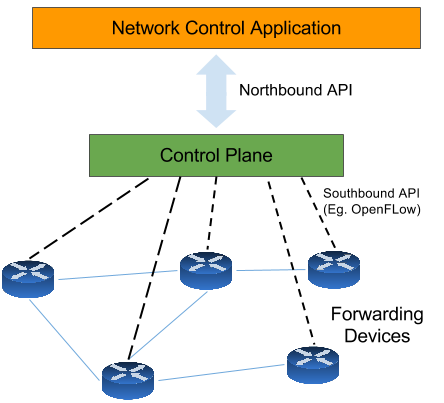
\includegraphics[scale=0.50]{SDNOverview.png}}
\caption{Fundamental abstractions of SDN.}
\label{Sec:SDNOverview}
\end{figure}

SDN allows the control of all forwarding devices in the network from a global vantage point; it achieves this by separation of the control plane from the data plane of the forwarding devices, enabling centralized control of the network \cite{mckeown2011sdn}. Moreover, it maintains the global state of the network and is responsible for the routing protocols being used in the network, enabling prototyping of new flow scheduling mechanisms. A high level overview of the SDN architecture is illustrated in Figure \ref{Sec:SDNOverview}. SDN allows for network programmability by installing flows in the switches, based on control logic that sits in a centralized controller which has a global view of the network. Hence, network applications can be developed which aim to maximize throughput by creating a tight-coupling between network flow scheduling and application communication patterns.  

Consequently, using SDN, the data centre network can be optimized to handle the traffic patterns of big data applications in topologies with path diversity, without being limited by traditional routing protocols which are insufficient to handle such communication patterns. 

\section{Project Motivation}

The motivation behind the current project is to device a flow scheduling approach in accordance with \textit{big data} application patterns, in particular MapReduce \cite{dean2008mapreduce}, which is \textit{proactive} in nature, so that the data centre network achieves maximum throughput and the application performs better. Existing research focuses on dynamic configuration of data centre networks by \textit{reactively} scheduling flows at application runtime. Our goal is to investigate if there are performance gains in terms of the total bisection bandwidth achieved by hosts running big data applications in the network, when the network is optimized \textit{proactively} based on application traffic patterns. 

By taking a global view of the network using SDN, we preconfigure the scheduling system in order to avoid bottlenecks and minimize control traffic overhead in the network. We use Hadoop \cite{HadoopWeb} as the application for proactive network integration due to it's widespread use and popularity. 

\section{Project Aims}
We propose a \textit{Proactive} approach for the configuration of a data centre network, which installs flow rules in the network before the big data application starts. In particular, we intend to 
\begin{itemize}
\item Determine whether there is an increase in the total bisection bandwidth achieved by the hosts in the network when flows are scheduled \textit{proactively}.  
\item Investigate the effectiveness of \textit{proactive} network configuration by comparing the Hadoop job completion times with \textit{reactive} flow scheduling approaches and static Equal Cost Multi-Path (ECMP \cite{hopps2000analysis}) routing.
\item Determine if there is an inverse correlation between total bisection bandwidth achieved and Hadoop job completion times for different flow scheduling strategies.  
\end{itemize}
\section{Project Approach}
We present a design of our \textit{Proactive} flow scheduler based on python, which leverages the flow scheduling decisions made by Global First-Fit \cite{al2010hedera} flow scheduling algorithm. Subsequently, we analyse the performance of our \textit{Proactive} flow scheduler against ECMP routing and Global First-Fit flow scheduling on an emulation based testbed.
\section{Document Structure}

Chapter \ref{chap:State} explores the current state-of-the-art in efforts to optimize data centre network traffic for big data applications using SDN, and the emulators used for prototyping novel network control logic. Chapter \ref{chap:Background} provides background for the project, explaining the working of MapReduce and its implementation in Hadoop, subsequently describing current state-of-the-art in data centre topologies such as the \textit{fat-tree topology} \cite{al2008scalable}, and finally providing an overview of ECMP routing and Global First-Fit flow scheduling which are used for evaluating our \textit{Proactive} flow scheduling. Chapter \ref{chap:design} describes the design of our \textit{Proactive} flow scheduler and gives a functional architectural overview of our experimental setup. The actual implementation of the design is described in Chapter \ref{chap:Implmentation}. Chapter \ref{chap:eval} details the benchmark tests used for evaluating our \textit{Proactive} flow scheduler against ECMP routing and Global First-Fit flow scheduling and provides a brief analysis on the results obtained. Finally, Chapter \ref{chap:conc} contains our concluding remarks.  
                                
  \chapter{State-of-the-Art} \label{chap:State}

In the previous chapter, we introduced our project, including our project motivation and aims. In this chapter, we describe the current state-of-the-art in the research area where our project lies and discuss relevant technologies and concepts upon which the current project is built. In Section \ref{sec:SDN}, we discuss the concept of Software-Defined Networking, which is the fundamental building block of our project. Subsequently, in Section \ref{sec:HadoopTraffic}, we analyse and contrast studies that have used Software-Defined Networking to optimize Hadoop application traffic, on the basis of which, the current project is based. And finally, in Section \ref{sec:Emulators}, we describe emulators used for emulating data centre networks and Hadoop jobs respectively, which have made this project possible. 

\section{Software-Defined Networking} \label{sec:SDN}

Fast paced innovations in Computing have accelerated the growth and adoption of technology throughout the world in every sphere of life. However, innovations in Computer Networking have not been very steady, part of it was because of the unwillingness to conduct experiments in a network carrying production traffic. Moreover, there were a large number of protocols and network equipment already deployed in the network, which made it more difficult to innovate \cite{mckeown2008openflow}. 

Software-Defined Networking (SDN) enables controlling of the entire network through a centralized controller which maintains state of the entire network and is responsible for functions such as the routing protocols used by the forwarding devices in the network \cite{lantz2010network}. SDN achieves this by separating the control plane from the forwarding plane, where the control plane is housed in the centralized controller, and the forwarding plane is controlled via a narrow channel such as the OpenFlow protocol \cite{mckeown2008openflow}, as illustrated in Figure \ref{fig:OpenFlowOverview}. Communication between the OpenFlow switches and the centralized controller is achieved over a secure channel which is encrypted via SSL. 
\begin{figure}[!ht] 
	\centerline{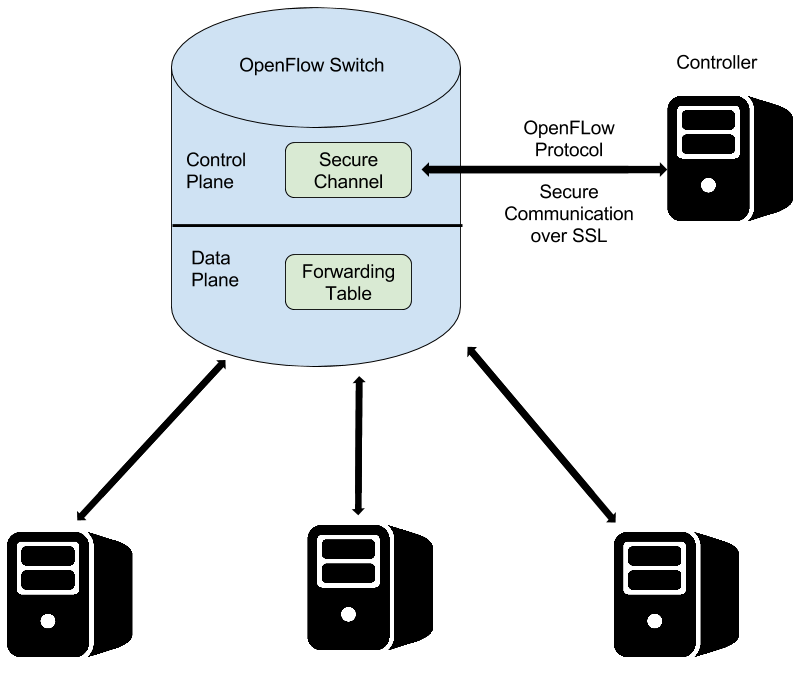
\includegraphics[scale=0.33]{graphics/chapter2/OpenFlowProtocol.png}}
	\caption{Overview of the operation of the OpenFlow protocol, where forwarding behaviour of switches is controlled by a centralized controller via a secure channel.}
	\label{fig:OpenFlowOverview} 
\end{figure}

Consequently, new functionality can be added in networks that are already deployed without any modification to the switches, and prototyping of new ideas can be conducted  without disrupting production traffic, enabling innovation in networking at software speeds \cite{lantz2010network}. 

SDN has resulted in a significant amount of research conducted with the aim of optimizing routing protocols and managing the network more efficiently \cite{kreutz2015software}. Examples of SDN Networks include FlowVisor \cite{sherwood2010carving}, PortLand \cite{niranjan2009portland} and Ethane \cite{casado2007ethane}. In this project, we leverage SDN to optimize data centre networks for Hadoop \cite{HadoopWeb} traffic. 
%\pagebreak
\section{Hadoop Traffic Optimization using SDN} \label{sec:HadoopTraffic}


\begin{table}[!ht]
\caption{Comparison of various studies that attempt to optimize data centre traffic of applications such as Hadoop using SDN} 
	\begingroup 
	\setlength{\tabcolsep}{5pt} % Default value: 6pt
	\renewcommand{\arraystretch}{1.2} % Default value: 1, use it to increase decrease padding
	\centerline{\begin{tabular}{|>{\columncolor[gray]{0.8}}L{2.2cm}|L{2.4cm}|L{2.4cm}|L{2.4cm}|L{2.4cm}|L{2.4cm}|} 
			\hline
			Study       & FlowComb \cite{das2013transparent} & Wang \textit{et al.} \cite{wang2012programming} & HybridTE \cite{wette2015hybridte} & Pythia \cite{neves2014pythia} & Hedera \cite{al2010hedera}  \\ \hline
			Approach    & Reactive & Reactive & Semi-Proactive & Reactive & Reactive \\ \hline
			Methodology & Software agents on every node report  demands, used to route traffic & Interface SDN controller with Hadoop master,which reports demands to controller & Install mice flows proactively and elephant flows reactively & Hadoop middleware predicts future transfers, network arranged accordingly  & Devised new flow scheduling algorithms as an extension to ECMP \\ \hline
			Uses Hadoop Traffic & Yes &  Yes & No & Yes & Yes \\ \hline 
			Result      & Reduced Hadoop Runtime by 33\% & Proposal, No Results & Outperforms Hedera and ECMP in flow completion times & Reduced Hadoop runtime by 43\% compared to ECMP & 39\% better bisection bandwidth achieved for Hadoop shuffle phase, compared to ECMP \\ \hline
			Limitations & Agents cause computational overhead, require domain specific knowledge & Requires creating demand estimator, computational overhead on master node & Underutilizes path diversity for mice flows, elephant flow detection suffer latencies & Domain-specific, intrusive to app data, induces computational overhead & 100ms latency in Scheduling due to control overhead, might increase when scaled to millions of hosts  \\ \hline 
			Type & Application-Aware & Application-Aware & Application-Aware & Application-Aware & Traffic-Aware  \\ \hline 
			\end{tabular}} 
		\endgroup
		\label{table:StudiesComparison}
\end{table}

In this section, we review various recent studies \cite{das2013transparent, wang2012programming, al2010hedera, narayan2012hadoop, neves2014pythia, wette2015hybridte} that have been conducted with the aim of optimizing application traffic of Big Data processing applications such as Hadoop \cite{HadoopWeb} (described in detail in \ref{subsec:HadoopOverview}), in a data centre network using SDN; in order to achieve faster data processing times through high network utilization. We give a high level overview and comparison of these studies in Table \ref{table:StudiesComparison}. Most of the work done in this area uses \textit{reactive} measures for data centre network configuration, which motivated us to explore a \textit{proactive} approach, as described in Chapter \ref{chap:design}. 

All the studies compared in Table \ref{table:StudiesComparison} employ \textit{multi-rooted} tree topologies, which are described in detail in \ref{sec: DataCentreArch}, while they compare their performance against Equal Cost Multi-Path (ECMP) \cite{hopps2000analysis} routing, which is the industry standard protocol for routing traffic in a multi-rooted tree topology having path diversity. ECMP is described in detail in \ref{subsec:ECMP}. All approaches to optimize Hadoop traffic using SDN can be broadly classified into \textit{Application-Aware networking} and \textit{Traffic-Aware Networking}. Studies employing the two approaches are discussed in the next subsections.

\subsection{Application-Aware Network Optimization} \label{subsec:AppAware}

\begin{figure}[!ht] 
	\centerline{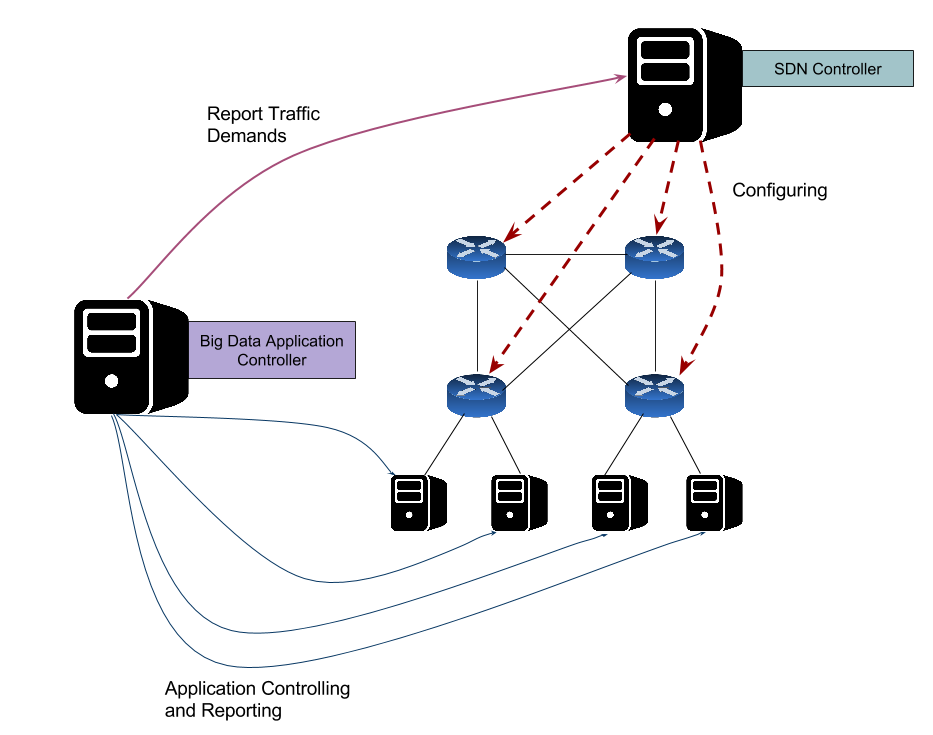
\includegraphics[scale=0.40]{graphics/chapter2/ApplicationAwareScheduling.png}}
	\caption{The big data application controller reports traffic demands to the network controller, enabling \textit{Application-Aware} flow scheduling.}
	\label{fig:ApplicationAwareScheduling}
\end{figure}

Figure \ref{fig:ApplicationAwareScheduling} illustrates the approach of \textit{Application-Aware} scheduling in order to optimize the network for Big Data applications. It attempts to tightly integrate Big Data application controllers with the SDN controller responsible for scheduling of flows in the network. The application controller reports traffic demands to the SDN controller on the bases of information obtained from the hosts, which is used by the SDN controller to configure forwarding devices in the network in a \textit{reactive} manner. We further discuss this approach of network optimization by analysing studies that are based on this methodology for network optimization.
 
Das \textit{et al.} \cite{das2013transparent} attempted to optimize Hadoop by introducing a network management framework called \textit{FlowComb} that leverages SDN and monitoring of all servers running Hadoop, to perform dynamic scheduling of flows.  

The main objectives of \textit{FlowComb} were to predict the network demand of an application in advance and dynamically install flows in the network switches based on its prediction. Das \textit{et al.} argued that studies monitoring the network to detect changes such as \textit{Hedera} \cite{al2010hedera}, do so only after a change has occurred; moreover network monitoring is an expensive operation. In order to anticipate network demands, Das \textit{et al.} developed software agents which were installed on all servers running Hadoop in a cluster. The Software agents essentially performed two functions, namely, scanning Hadoop logs to extract information about map tasks and network transfers; and sending this information to the scheduling component of \textit{FlowComb}, which is the SDN controller, thereby making the SDN controller \textit{application-aware}. 

Similar to Hedera \cite{al2010hedera} as described in \ref{subsec:Hedera}, \textit{FlowComb's} Scheduling engine dynamically allocates and installs paths in the network using the OpenFlow protocol \cite{mckeown2008openflow}; in order to avoid traffic congestion and provide sufficient bandwidth to all flows. \textit{FlowComb} was found to reduce the average running time of sorting 10 GB of data in a 14 node Hadoop cluster by \textit{33\%} \cite{das2013transparent}. 

\textit{FlowComb} has a number of drawbacks, such as it depends on domain-specific knowledge to operate, hence the same implementation of \textit{FlowComb} cannot be applied to different MapReduce implementations apart from Hadoop \cite{HadoopWeb}, such as Dryad \cite{isard2007dryad} and Spark \cite{SparkWeb}. Furthermore, since reducers start transfers at random, \textit{FlowComb} cannot determine the exact timing of the start of a transfer \cite{das2013transparent}; extracting information at the hosts by scanning Hadoop logs causes a computation overhead and finally, \textit{FlowComb} helps in optimizing Hadoop jobs only when the network is congested. 

Similarly, Wang \textit{et al.} \cite{wang2012programming} have proposed to tightly integrate Big Data applications with network control by leveraging the programmability of networks provided by SDN and the high network bandwidth provided by optically switched networks, making the network \textit{application-aware}. Since applications such as Hadoop \cite{HadoopWeb} have a master node that maintains an overall control over the other nodes in a cluster, as described in \ref{subsec:HadoopOverview}, Wang \textit{et al.} suggest to interface the SDN controller with the master node, thereby enabling application controllers to report traffic demands to the SDN controller and issue topology configuration commands to the SDN controller, on the basis of which, the network is configured \textit{reactively}.

The approach suggested by Wang \textit{et al.} \cite{wang2012programming} would have to overcome a number of challenges. A demand estimator engine would need to be implemented for every application that has to be interfaced with the SDN controller for the master node, which would introduce a significant computational overhead for the master node \cite{wang2012programming}. The \textit{reactive} nature of configuring the topology at runtime, as suggested by Wang \textit{et al.} imposes significant computational responsibilities on the SDN controller to re-configure the network in response to traffic demands with low latency, and imposes a challenge on the SDN controller's scalability.

Wette \textit{et al.} \cite{wette2015hybridte} argue that \textit{reactive} approaches such as Hedera \cite{al2010hedera}, which try to optimize data centre networks by reactively installing flow entries, overwhelm the switching hardware by the number of flows that they tend to install. In order to alleviate overwhelming of switching hardware, Wette \textit{et al.} propose a \textit{semi-proactive} approach of flow scheduling called \textit{HybridTE}. By exploiting explicit knowledge about elephant flows, \textit{HybridTE} is able to perform flow scheduling using very few flow entries in the switches. \textit{HybridTE} treats mice flows and elephant flows differently, by installing flow entries \textit{proactively} for mice flows  and \textit{reactively} for elephant flows. 

Using a data centre architecture as described in \ref{sec: DataCentreArch}, \textit{HybridTE} installs one forwarding tree per ToR switches using OpenFlow wild-card flow table entries in a \textit{proactive} manner, which, Wette \textit{et al.} argue is sufficient for small flows. As far as the elephant flows are concerned, Wette \textit{et al.} investigate the effect of different techniques for elephant flow detection such as HadoopWatch \cite{peng2014hadoopwatch}, which monitor Hadoop logs to predict upcoming file transfers and packet sampling, which has been demonstrated by Choi \textit{et al.} \cite{choi2004adaptive} to be effective in determining elephant flows when using a reasonable sample. Using elephant flow detection schemes as previously described, \textit{HybridTE} re-routes elephant flows to the shortest path which is the least congested, in a \textit{reactive} manner. 

\textit{HybridTE} was found to outperform ECMP \cite{hopps2000analysis} and Hedera \cite{al2010hedera} in terms of flow completion times, with ECMP taking 29.1\% longer times for flow completion in a network with increasing congestion than \textit{HybridTE} \cite{wette2015hybridte}. However, \textit{HybridTE} has certain limitations such as it does not exploit path diversity for routing mice flows, and detecting elephant flows to avoid congestion has inherent high-level latencies.  

\textit{Pythia} \cite{neves2014pythia} is another study that aims to optimize Hadoop job completion times by predicting Hadoop data transfers at runtime and avoiding congestion during the Hadoop shuffle phase by dynamically routing network flows. \textit{Pythia} has two components

\begin{itemize}
	\item Hadoop instrumentation middle-ware that runs on all of the Hadoop worker nodes, responsible for predicting future shuffle transfers by extracting information from Hadoop logs, similar to software agents employed by FlowComb \cite{das2013transparent}.
	\item An Orchestration entity that dynamically allocates reactive paths on runtime on the basis of future shuffle transfers predicted by the middle-ware which is sent to it. 
\end{itemize} 

The Hadoop instrumentation middle-ware is able to determine the size of a data transfer, since after a map task finishes, it writes the intermediate $<$key, value$>$ pairs to disk \cite{narayan2012hadoop}, which is read by the instrumentation middle-ware \cite{neves2014pythia}. The size of the future transfer, along with the map task ID is subsequently transmitted to the orchestration controller, which \textit{reactively} configures the network based on the supplied prediction.  

Neves \textit{et al.} evaluated \textit{Pythia} on a cluster of 10 servers with a total RAM of 128GB and found that \textit{Pythia} outperforms ECMP which is the industry standard for multipath routing, as explained in \ref{subsec:ECMP}; by lowering Hadoop job completion times by 43\% \cite{neves2014pythia}. However, \textit{Pythia} has certain limitations, such as the Hadoop instrumentation layer is able to access Hadoop logs, making it intrusive and difficult to implement in a multi-tenant data centre, with different Hadoop jobs running simultaneously causing a computational overhead at the worker nodes. \textit{Pythia} is very specific to Hadoop and would not function for a broader range of communication patterns. 

\subsection{Traffic-Aware Network Optimization}

In contrast to \textit{application-aware} network optimization, as discussed in \ref{subsec:AppAware}, \textit{traffic-aware} network optimization seeks to optimize the network by continuously monitoring forwarding devices and reporting the changing traffic information to the SDN controller, as illustrated in Figure \ref{fig:TrafficAwareScheduling}, which subsequently performs flow scheduling on the bases of the reported information. This monitoring can be done via the SDN controller itself, since it can request traffic statistics from OpenFlow switches. 

\begin{figure}[!ht] 
	\centerline{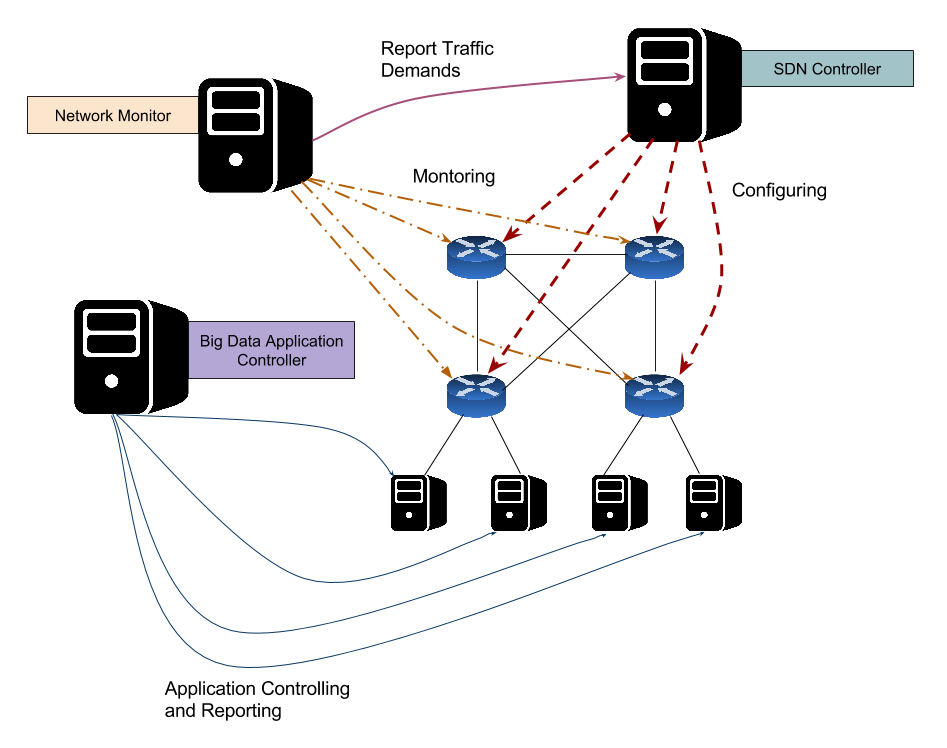
\includegraphics[scale=0.40]{graphics/chapter2/TrafficAwareScheduling.png}}
	\caption{The network is monitored continuously to keep track of traffic demands, enabling \textit{Traffic-Aware Scheduling}.}
	\label{fig:TrafficAwareScheduling}
\end{figure}

\textit{Hedera} \cite{al2010hedera} is one such study that employs \textit{traffic-aware} scheduling. The study proposes an extension to ECMP, whereby, it routes flows exceeding a certain threshold in a \textit{reactive} manner. We do a more comprehensive discussion on Hedera's Global First-Fit flow scheduling algorithm in \ref{subsec:Hedera} and evaluate implementations of ECMP and Global First-Fit against our \textit{proactive} approach in Chapter \ref{chap:eval}. \textit{Hedera} was found to significantly reduce Hadoop shuffle transfer times in comparison to ECMP routing, achieving 39\% more of the total bisection bandwidth available in the network, as compared to ECMP.

\section{Emulators for Data Centre Experimentation} \label{sec:Emulators}

In this section, we describe the emulators that we used for the implementation of our current project, detailed in Chapter \ref{chap:Implmentation}, since we did not have access to a cluster of servers for running our experiments. Firstly, in \ref{subsec:DataCentreEmulation}, we describe the emulator used for emulating data centre networks and subsequently, in \ref{subsec:Mremu} we describe an emulator that emulates the working of Hadoop \cite{HadoopWeb} using real Hadoop traces.  

\subsection{Data centre Network Emulation}  \label{subsec:DataCentreEmulation}
In order to exploit the full potential of SDN as described in \ref{sec:SDN}, it should be possible to prototype novel approaches for network control without the need of running experiments in a data centre, since all researchers do not have access to such resources. Lantz \textit{et al.} \cite{lantz2010network} filled this gap by introducing \textit{Mininet}, which is a lightweight virtualization platform for prototyping SDN Networks. \textit{Mininet} can work on the constraint resources of a single laptop. It is built with the following attributes
\begin{itemize}
	\item Allows defining of new topologies and functionality using familiar programming languages, specifically, python \cite{van2007python}.
	\item Network can be deployed from virtual to physical hardware without any change in code, with high degree of fidelity in behaviour. 
	\item Allows managing the network in real time, scaling to thousands of switches on a single physical host. 
\end{itemize} 

Code created in other similar emulators like Opnet \cite{opnetWeb} and ns-2 \cite{ns2} for network simulation cannot be ported directly to real hardware; moreover, they don't provide the functionality of interacting with the network in real time \cite{lantz2010network}. On the other hand, \textit{Mininet} leverages Linux features such as network namespaces and virtual Ethernet pairs, enabling it to offer support for networks with bandwidth in Gigabits and hundreds of nodes such as controllers, switches and hosts; all of which are emulated with ease on a single laptop. All these attributes made \textit{Mininet} the ideal choice of network emulator for our current project since we did not have access to a cluster of servers.

\textit{Mininet} combines its lightweight Linux virtualization with an interactive command line interface and an extensible API written in python to experiment with SDN. The interactive CLI can be used to manage the entire SDN network from a single command line while a simulation is running. The \textit{Mininet} python API can be used to define custom network topologies, node types and experiments \cite{lantz2010network}.

\textit{Mininet} uses Open vSwitch \cite{OpenvSwitch} for emulating OpenFlow switches in the network, and works well with all SDN controllers such as POX/NOX \cite{gude2008nox}, OpenDayLight \cite{ODL2016}, \textit{et cetera}. A \textit{Mininet} host is essentially a shell process which resides in it's own namespace \cite{lantz2010network}, having virtual Ethernet interfaces,  making it very lightweight. An SDN controller can work with \textit{Mininet} as long as the switches running in mininet have IP connectivity to the controller \cite{lantz2010network}.

\textit{Mininet} scales well to over 1000 nodes owing to sharing of the file system, process ID space, kernel and other resources, providing a bandwidth of 1-3 Gbps through a single switch \cite{lantz2010network}, making it ideal for running emulations of a data centre network on a single laptop. However, \textit{Mininet} has certain limitations, such as it suffers from a lack of performance fidelity when the emulation has high loads, additionally, software based forwarding cannot surpass the speeds obtained by TCAM accelerated vendor switches, live host migration is not supported and \textit{Mininet} does not support distributed emulation since it can only run on a single machine. Nonetheless, \textit{Mininet} offers a viable alternative to running experiments in real hardware and provides a scalable and interactive environment with an extensible API to conduct experiments, which is why we chose it for implementing our experiment as described in Chapter \ref{chap:Implmentation}.  


\subsection{Hadoop Emulation} \label{subsec:Mremu}

Use of real hardware robust enough for running data centre experiments is not a valid option for many researchers since such resources are not readily available. We faced a similar problem, therefore we chose to run the experiments of this project on a Hadoop emulator-based test bed.   

The emulator that met our requirements was MRemu, devised by Neves \textit{et al.} \cite{neves2015mremu}. MRemu is a framework that works as a Hadoop emulator by reproducing traffic patterns of a Hadoop job trace with the same latencies as in the original Hadoop job trace. Hence, using MRemu, Hadoop jobs are emulated in hosts running on Linux containers \cite{neves2015mremu} such as \textit{Mininet}, as described in \ref{subsec:DataCentreEmulation} to emulate data centre nodes, running on a single physical host, which have low IO and CPU resources to run a real Hadoop job.

Studies have demonstrated that MapReduce applications are sensitive to performance of the network \cite{das2013transparent, chowdhury2011managing}, nonetheless, numerous studies use synthetic traffic patterns, generated following certain probabilistic distributions \cite{al2008scalable, greenberg2009vl2, curtis2011devoflow}, which fails to capture the true network workloads \cite{neves2015mremu}. Taking this into consideration, Neves \textit{et al.} developed a tool for extracting traces from Hadoop job execution logs with enriched network information to generate comprehensive Hadoop job traces to be used with MRemu. These traces \cite{MRemuRepo2015} produced by Neves \textit{et al.}, made available online, have been employed by us in this project. 

\begin{figure}[!ht] 
\centerline{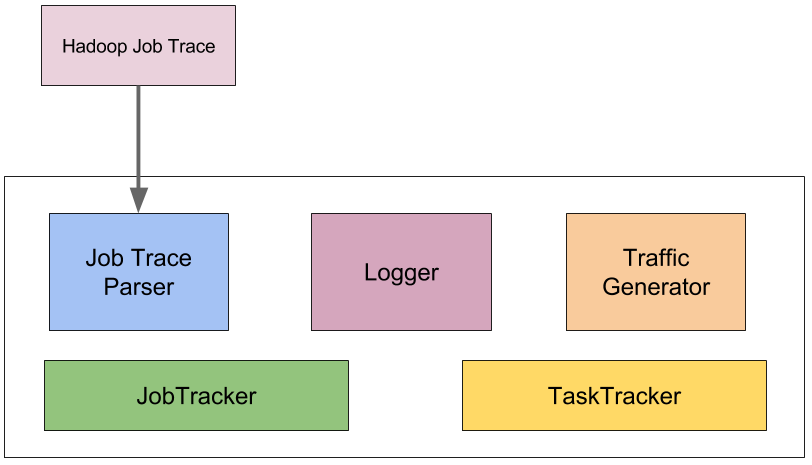
\includegraphics[scale=0.30]{MRemuOverview.png}}
\caption{Block Diagram of MRemu Hadoop Emulator.}
\label{fig:MRemuOverview}
\end{figure}

Figure \ref{fig:MRemuOverview} shows a high level overview of the Hadoop emulator in MRemu. Hadoop job traces are fed to the Job Trace parser, which uses information from the trace, such as wait times and task durations, to mimic the latencies in a real Hadoop job execution. The traffic generator generates \textit{iperf} flows, mimicking network transfers of the real Hadoop job corresponding to the trace, while the logger logs Hadoop events to local disk of the emulated nodes.  

MRemu makes it possible to test different network routing control logic using SDN for Hadoop traffic on the constraints of a single physical system, making it ideal to be used in conjugation with \textit{Mininet}, as described in \ref{subsec:DataCentreEmulation}, for Hadoop traffic scheduling experimentation. MRemu supports production SDN controllers such as POX/NOX \cite{gude2008nox} and OpenDayLight \cite{ODL2016}, making it ideal for evaluating novel approaches to route Hadoop traffic in order to accelerate it. 

Neves \textit{et al.}  \cite{neves2015mremu} tested MRemu, by first obtaining Hadoop traces from a real cluster of 16 identical nodes, running Hadoop 1.1.2, while the emulation was performed on a single node with 16 GB of RAM and 16 x86 64 cores, running on \textit{Mininet} 2.1.0. The original Hadoop jobs ran applications forming part of the HiBench Benchmark Suite \cite{huang2011hibench} such as Bayes, Sort, Nutch and PageRank. On performing a comparison between job completion times in real hardware and the MRemu emulation setup, Neves \textit{et al.} observed that the job completion times were comparable. Furthermore, Neves \textit{et al.} evaluated individual flow completion times as well and found the transfer durations in the emulation to be slightly different than the real transfer durations, owing to inaccuracies in Hadoop logs (used to extract traces) due to high-level latencies. Nonetheless, Job Completion times were found to be near accurate, owing to which, we chose to use MRemu for evaluating our proactive approach as described in Section \ref{chap:Implmentation}. 

However, MRemu has certain limitations, such as 

\begin{itemize}
\item MRemu supports emulation of only one job at a time, having no support of concurrent job execution. 
\item MRemu does not model failure handling techniques of Hadoop, making it a requirement of only running successful job traces for emulation \cite{neves2015mremu}.
\item MRemu does not support distributed emulation, hence it can only support a limited number of Linux container nodes that can be supported by a single physical server and cannot scale to hundreds of nodes. 
\end{itemize}

Nonetheless, MRemu adequately met our requirements for a Hadoop emulator that can be run over \textit{Mininet}, therefore, we chose to use it for the current project in conjugation with \textit{Mininet}.
 

                                
  \chapter{Background} \label{chap:Background}

In this chapter, we describe the research which led to the current project. In Section \ref{sec:MapReduce}, we provide an overview of the MapReduce framework and subsequently the Hadoop MapReduce implementation \cite{HadoopWeb}.  

Furthermore, in Section \ref{sec: DataCentreArch} we describe the current state-of-the art in data centre architecture design and focus on  \textit{fat-tree} \cite{al2008scalable} data centre topology in \ref{subsec:Fat-Tree Topology}, which is used in our experiment as the network topology because of its ability to alleviate inter-node communication bandwidth bottlenecks in large-scale clusters. 

Finally, in Section \ref{sec:Flow Scheduling in Data Centres} we describe the current state-of-the-art \textit{flow scheduling} mechanisms for in data centre networks, namely Equal Cost Multi-Path Routing (ECMP \cite{hopps2000analysis}) and Global First-Fit \cite{al2010hedera}, implementations of which are used in our experiment to compare against proactive measures of flow scheduling.   

\section{MapReduce} \label{sec:MapReduce}

\begin{figure}[!ht]
\centerline{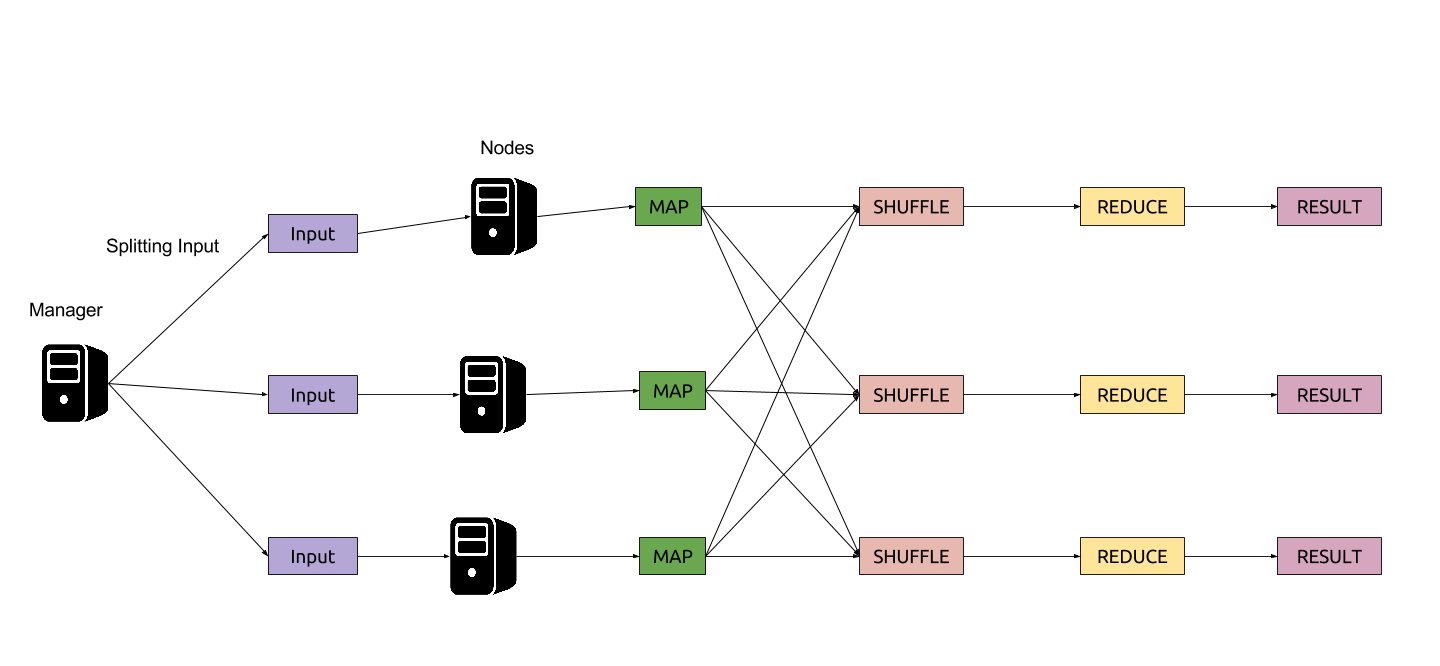
\includegraphics[scale=0.30]{GeneralMapReduce.png}}
\caption{High level overview of the MapReduce Framework.}
\label{fig:MROverview}
\end{figure}

MapReduce was introduced by Dean \textit{et al.} \cite{dean2008mapreduce} as a programming abstraction, which enables distributed cluster computing with commodity servers and is highly fault tolerant and reliable. MapReduce is one of the most frequently used framework for big data processing \cite{barroso2013datacenter} and we chose it for our project due to its ubiquity and popularity. It broadly consists of 3 phases, namely the \textit{map}, \textit{shuffle} and \textit{reduce} phases as illustrated in Figure \ref{fig:MROverview}. 
  
MapReduce is a computational model based on \textit{key-value} pairs. The \textit{Map} function produces a set of intermediate \textit{key-value} pairs for a given input \cite{dean2008mapreduce}. Subsequently, the intermediate data is grouped according to its keys in the \textit{shuffle} phase. Finally, in the \textit{reduce} phase, all values for a given key are combined to produce the final result. The data used for MapReduce jobs is usually stored in a distributed file system (DFS), which takes care of fault tolerance by replicating the data across the cluster. Examples of such data stores include GFS \cite{ghemawat2003google} and HDFS \cite{borthakur2008hdfs}.

\subsection{High Level Execution Overview} \label{subsec:MROverview}

The input data set of a MapReduce job is first partitioned into \textbf{M} pieces, which are processed in parallel by different machines \cite{dean2008mapreduce}. The Reduce function is invoked by partitioning the intermediate key set of the data into a set of \textbf{R} pieces, which is distributed across the entire cluster for computation. 

MapReduce computation proceeds in the following steps

\begin{itemize}
\item The input file is first split into \textbf{M} pieces while MapReduce starts up on the entire cluster of machines.
\item One of the machines in the cluster is designated as the \textit{master} node, while all the other nodes in the network are \textit{worker} nodes which are assigned jobs by the \textit{master} node. The master assigns a map task or a reduce task to each one of the idle worker nodes in the network from a total of \textbf{M} map tasks and \textbf{R} reduce tasks.
\item The corresponding partitioned input is read by the worker which is assigned a map task, it parses the input and emits key-value pairs and passes each of those to the map function. Intermediate key-value pairs emitted by the map function are buffered in memory.
\item The buffered pairs are written into persistent memory store of the worker nodes on a periodic basis and are partitioned into \textbf{R} pairs. Memory locations of these key-value pairs are sent to the master node so that they can be forwarded to the reduce worker nodes \cite{dean2008mapreduce}.
\item On notification about these locations, the reduce worker reads the buffered data from the persistent memory store of the map workers via RPC calls \cite{dean2008mapreduce}. Subsequently, it sorts the intermediate keys of the data by grouping the same keys together, this is also called the shuffling phase. 
\item  The sorted intermediate data is iterated upon by the reduce worker nodes and for each unique key encountered, it passes the corresponding key-value pairs to the reduce function. 
\end{itemize}

After all the above steps culminate, the output consists of \textbf{R} output files. These files may or may not be merged into a single output file, depending on the MapReduce implementation. 

\subsection{Hadoop Overview} \label{subsec:HadoopOverview}

Hadoop is one of the most frequently used open source MapReduce implementations. We choose Hadoop as the MapReduce implementation of choice for this project due to it being open source and its widespread usage for Big Data analysis. It broadly consists of \textit{two} main components   
\begin{itemize}
\item Hadoop MapReduce - Open-source implementation of the MapReduce computation model.
\item HDFS (Hadoop Distributed File System) - A resilient, fault tolerant and distributed file system that provides high throughput access to application data and is designed to be used with commodity hardware \cite{borthakur2008hdfs}.
\end{itemize}
\begin{figure}[!ht]
\centerline{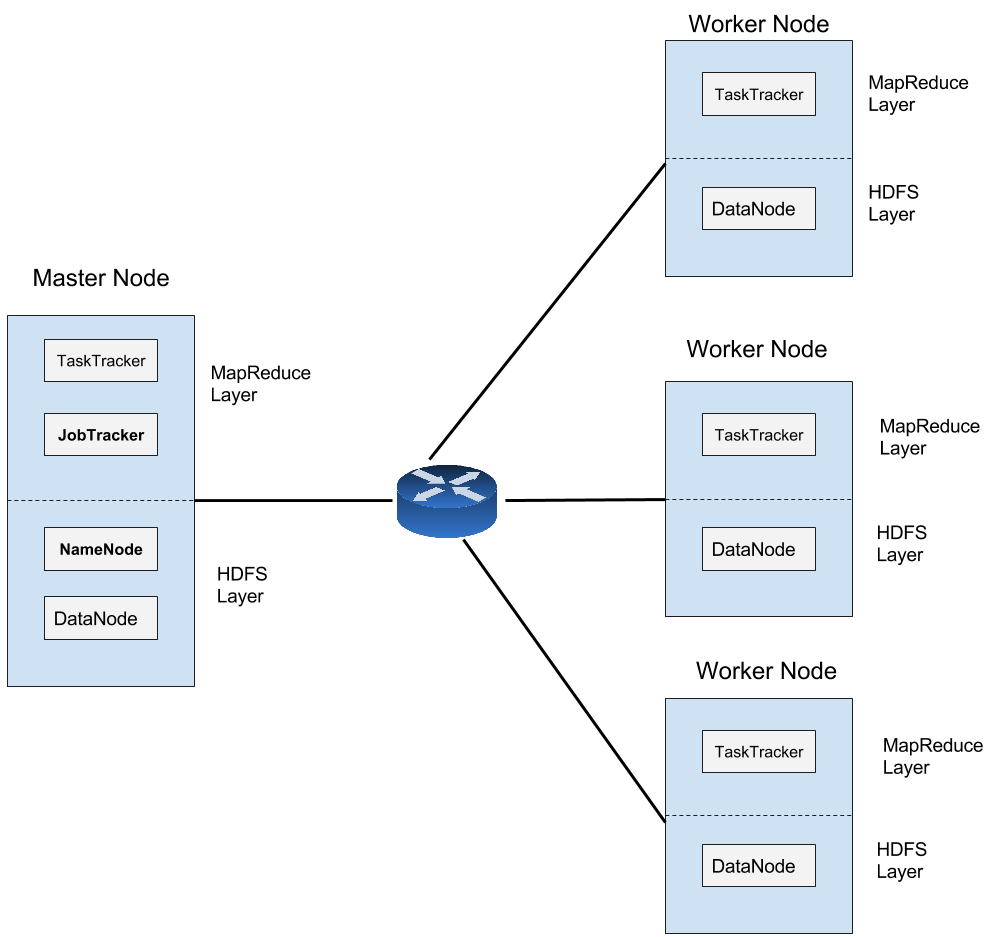
\includegraphics[scale=0.35]{HadoopArchitecture.png}}
\caption{Basic Hadoop Architecture with the master node housing the JobTracker and the NameNode functionalities of Hadoop, while the worker (slave) nodes housing the TaskTracker and DataNode functionalities of Hadoop.}
\label{fig:HadoopArchitecture}
\end{figure}

Similar to the Google MapReduce model \cite{dean2008mapreduce} outlined in Section \ref{sec:MapReduce}, HDFS too has a master-slave architecture \cite{borthakur2008hdfs}. As illustrated in Figure \ref{fig:HadoopArchitecture} a Hadoop cluster consists of the following
\begin{itemize}
	\item HDFS layer consists of two types of nodes responsible for managing the Distributed file system 
    	 \begin{itemize}
		  \item \textbf{NameNode} - The entire Hadoop cluster contains one \textit{NameNode} which serves as the master server, managing the file system access of worker nodes and the file system name space. It also instructs the \textit{DataNodes} (slaves) in the cluster to create, delete and replicate data blocks.
		  \item \textbf{DataNode} - There is a usually one \textit{DataNode} on each node in the cluster, which is responsible for managing the persistent storage attached to that node in the cluster. File system read and write requests are also processed by the \textit{DataNodes}.    
		  \end{itemize}
    \item MapReduce layer consists of two types of nodes that control the execution of MR jobs \cite{white2012hadoop} 
    	 \begin{itemize}
		  \item \textbf{JobTracker} - Similar to the \textit{NameNode}, there is one \textit{JobTracker} Node in a Hadoop cluster, housed in the master node, which is responsible for scheduling all the jobs of the system to be run on the \textit{TaskTracker} (worker) nodes \cite{white2012hadoop}. It keeps track of the progress of every job, rescheduling it to other \textit{TaskTracker} nodes in case of failure \cite{white2012hadoop}. 
		  \item \textbf{TaskTracker} - \textit{TaskTrackers} or worker nodes, run the MR jobs assigned to them by the \textit{JobTracker} node and report the progress back to the \textit{Jobtracker} \cite{white2012hadoop} node. 
		  \end{itemize}
\end{itemize}

Most of the data transfer loads in a Hadoop cluster are attributed to the shuffling phase, when intermediate data from the mappers is shuffled over to the reducer nodes, as outlined in subsection \ref{subsec:MROverview}. 

Chowdhury \textit{et al.} \cite{chowdhury2011managing} analysed Hadoop traces from Facebook's Hadoop cluster and found that on an average, 33\% of the runtime is consumed by the shuffle phase. Additionally, in 26\% of the tasks with reduce jobs, more than 50\% of the runtime is spent in the shuffle phase, while it accounts for upwards of 70\% of the runtime in 16\% of the jobs \cite{chowdhury2011managing}, confirming results reported in literature \cite{al2010hedera, greenberg2009vl2,guo2008dcell} which state that network is a bottleneck in MapReduce. Therefore, with this project, we aim to make the network \textit{application-aware} to alleviate loss in performance of MapReduce due to network bottlenecks.

\section{State-of-the-art in Data Centre Architectures} \label{sec: DataCentreArch}

Distributed big data computational frameworks such as MapReduce \cite{dean2008mapreduce}, Dryad \cite{isard2007dryad} and Hadoop \cite{HadoopWeb} leverage enormous clusters made up of commodity CPUs for their compute prowess. Various recent studies  \cite{benson2010understanding, chang2008bigtable, decandia2007dynamo, ghemawat2003google, greenberg2009vl2} have determined that networks are bottlenecks in data centres running distributed big data application frameworks. In order to scale the number of hosts in a cluster running these distributed big data application frameworks,  multiple paths are required between source and destination hosts  \cite{al2008scalable,greenberg2009vl2, greenberg2008towards, guo2008dcell,guo2009bcube}, which has heavily influenced data centre network design. 

Recent data centre architectures advocate horizontal scaling of hosts instead of vertical to overcome limited port densities in commercial switches in order to support the communication patterns of big data applications \cite{al2008scalable,greenberg2009vl2, greenberg2008towards}; therefore such architectures take advantage of the availability of a large number of parallel paths between any two source and destination switches, and are known as \textit{multi-rooted tree} topologies \cite{al2010hedera}. Multi-rooted tree topologies consist of two or three level trees of switches \cite{al2008scalable, al2010hedera} with higher speed links, while the aggregate bandwidth decreases while moving higher up in the multi-rooted tree topology \cite{headquarters2007cisco}.  

\begin{figure}[!ht] 
	\centerline{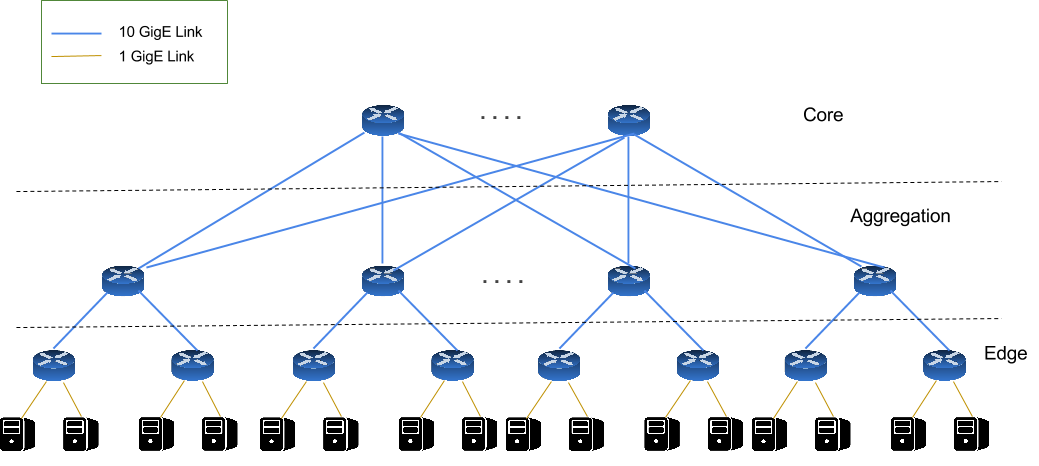
\includegraphics[scale=0.30]{Multi-rootedArch.png}}
	\caption{Common Multi-Rooted Data Centre Architecture with 10 GigE and 1 GigE links.}
	\label{fig:MultiRootedArch}
\end{figure}

At the leaf of a multi-rooted tree topology, there are a number of GigE ports (48-288) with 10 GigE uplinks to one or more switches in the \textit{aggregation layer} \cite{al2008scalable} as illustrated in Figure \ref{fig:MultiRootedArch}. Moving up in the tree hierarchy, switches have 10 GigE ports (32-128), capable of switching significant amounts of traffic between the edges \cite{al2008scalable}. 

Al-Fares \textit{et al.} \cite{al2008scalable} advocate the use of a \textit{fat-tree topology} \cite{leiserson1985fat} for data centre network design and showed that full aggregate bisection bandwidth can be achieved using commodity Ethernet switches of data centre clusters with tens of thousands of hosts. Fat-tree topology aims to alleviate shortcomings in current data centre network design such as

\begin{itemize}

\item over-subscription of links higher up in the topology, where over-subscription is defined by  Al-Fares \textit{et al.} \cite{al2008scalable} to be the ratio of worst-case aggregation bandwidth which can be achieved by the end hosts to the total bisection bandwidth available in the network; where typically, data centre designs are oversubscribed by a ratio of 2.5:1 (400 Mbps) to 8:1 (125 Mbps) with 1 Gb/s commodity Ethernet switches \cite{headquarters2007cisco} and,   

\item the cost of building a network with an over-subscription ratio of 1:1 is quite substantial, with each of the 48-port GigE switch at the edge costing around \$7000, while the 128-port switches at the aggregation and core layer cost around \$700,000 \cite{al2008scalable},
\end{itemize}

by providing backward compatibility to hosts running Ethernet and IP, scaling economically using commodity Ethernet switches for data centre design and providing a scalable interconnection bandwidth enabling any host to communicate with any other host in the network at it’s full local network interface bandwidth \cite{al2008scalable}.

\subsection{Fat-Tree Topology} \label{subsec:Fat-Tree Topology}

\textit{Fat-tree} topology \cite{leiserson1985fat} is a special instance of a \textit{Clos} topology, which was introduced in the 1950s to deliver high levels of bandwidth in telephone networks by interconnecting smaller commodity switches \cite{clos1953study}.  It is organised into \textit{k}-pods, where each pod contains of two layers of \textit{k}/2 switches \cite{al2008scalable}. Each of the \textit{k}/2 hosts in the lower layer are connected directly to each of the \textit{k} port switches in the lower layer of the pod. The remaining \textit{k}/2 ports of each of the switches in the lower layer are connected to \textit{k}/2 ports of the total \textit{k} ports up the hierarchy in the aggregation layer.

The core switches are $\textit{k}/2^2$ in number, with each of the core switch having one port connected to each of the \textit{k} pods . Consecutive ports in the aggregation layer of each pod switch are connected to core switches on \textit{k}/2 strides in such a manner that the ith port of any core switch is connected to pod i. A fat-tree topology built with k-port switches supports $\textit{k}^3/4$ hosts.


\begin{figure}[!ht] 
\centerline{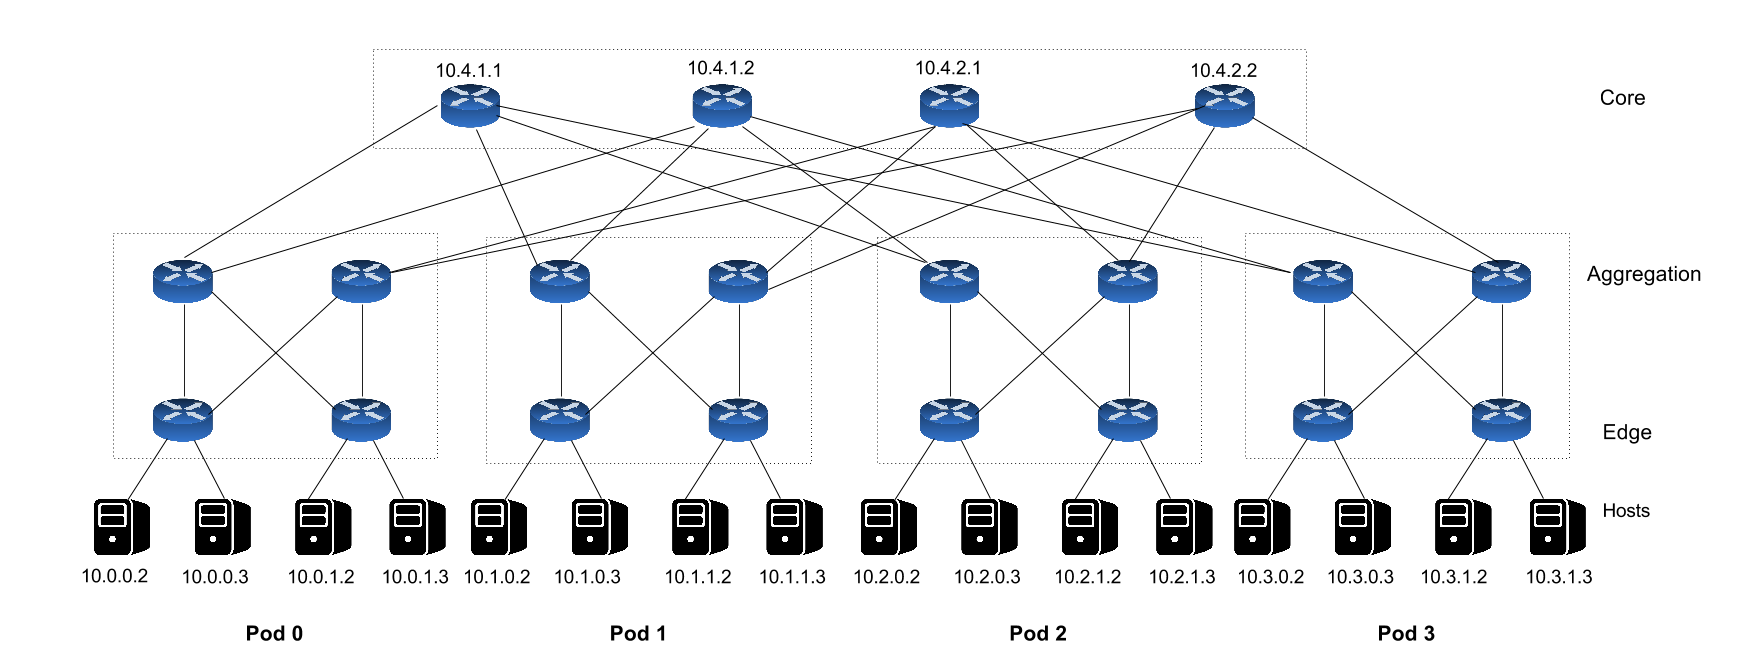
\includegraphics[scale=0.30]{FatTreeTopology.png}}
\caption{Fat-tree topology with 4 pods having 16 hosts in total (k=4).}
\label{fig:FatTreeOverview}
\end{figure}

In this project, we use a fat-tree topology with \textit{k} = 4 for our experiments as described in Chapter \ref{chap:design}. Figure \ref{fig:FatTreeOverview} illustrates a \textit{k}-ary fat-tree topology with \textit{k} = 4, which is the topology we  employ for our experiments. It consists of $\textit{k}^3/4$ i.e. 16 host machines with 4 pods. Hosts connected to the same lower level switch form a subnet; hence, all traffic between two hosts in the same subnet is switched while all the other traffic is routed.

In order to achieve maximum bisection bandwidth in a fat-tree network, outgoing traffic from a pod needs to be spread evenly amongst the core switches. There is a need for the core switches to be able to recognize and provide special behaviour to the traffic classes that need even spreading since  

\begin{itemize}

\item Routing protocols such as OSPF2 \cite{moy1998open} take hop-count as a metric of shortest path, causing switches to concentrate traffic going to a subnet to a single port even though there are $(\textit{k}/2)^2$ paths in the network with the same cost, thereby under utilizing the path diversity in the network and causing severe congestion at these points \cite{al2008scalable}.

\item Extensions to OSPF2 such as OSPF-ECMP \cite{thaler2000multipath} cannot be used on commodity Ethernet switches and require an overwhelmingly large number of prefixes.
 \end{itemize}

To alleviate these shortcomings, Al-Fares \textit{et al.}, devised an addressing scheme that allocates all IP addresses in the network within the private 10.0.0.0/8 block. 

Addressing in a \textit{fat-tree} topology follows the following pattern 

\begin{itemize}
	\item Switches in the pod are allocated IP addresses in the form 10.\textit{pod}.\textit{switch}.1, where \textit{pod} belongs in the range [0, \textit{k}-1], while the \textit{switch} denotes the position of the switch in the pod
	
	\item Core switches are allocated addresses in the form 10.\textit{k}.\textit{j}.\textit{i}, where \textit{j} and \textit{i} denote the co-ordinates of the core switch in the $(\textit{k}/2)^2$ grid 
	
	\item Hosts have addresses of the form 10.\textit{pod}.\textit{switch}.\textit{I D}, where \textit{I D} denotes the host's position in its subnet 
\end{itemize}

This addressing scheme helps in building a two-level routing scheme and scales to 4.2M hosts. The two-level routing scheme enables even spread of traffic across the network \cite{al2008scalable}. Two-level lookup is implemented in hardware using Ternary Contet-Accesible Memory (TCAM).

Due to all these optimizations, Al-Fares \textit{et al.} \cite{al2008scalable} found that in a fat-tree network of 16 hosts, the two-level switches achieve approx. 75\% of the aggregate ideal bisection bandwidth. For their benchmark suite, Al-Fares \textit{et al.} leveraged dynamic flow allocation strategies available in certain routers and found that their flow classifiers performed significantly better than traditional tree topologies which achieve only 28\% of the ideal bandwidth, with the worst-case aggregate bisection bandwidth achieved by the network to be 75\% of the ideal. In light of the results achieved by Al. Fares \textit{et al.}, we choose \textit{fat-tree} topology as the topology of choice for running our simulations described in Chapter \ref{chap:design}.

 
\section{Flow Scheduling in Data Centre Networks} \label{sec:Flow Scheduling in Data Centres}

To take advantage of topologies such as \textit{fat-tree}, described in \ref{subsec:Fat-Tree Topology}, which have multiple paths between the same host-destination pair. In this section, we describe current state-of-the art protocols such as Equal-Cost Multi-Path (ECMP) \cite{hopps2000analysis} and Hedera \cite{al2010hedera} for Multi-Path flow scheduling. These two flow scheduling techniques along with our \textit{proactive} approach are employed in the design of our experiment as described in Chapter \ref{chap:design} and subsequently evaluated against each other in Chapter \ref{chap:eval}.

\subsection{Equal Cost Multi-Path Routing} \label{subsec:ECMP}

Switches that support ECMP are configured with many possible paths for the same host-destination pair. When a packet arrives at a switch, with possible multiple paths to its destination, selected fields of the packet are hashed modulo the total no of paths and the packet is forwarded along the path that corresponds to the result. This results in splitting of the load, maintaining the arrival of packets for the same flow. ECMP is supported by most enterprise switches.

However, ECMP has a lot of limitations, such as it does not take flow bandwidth into account when it makes flow allocation decisions, which can cause bottlenecks at certain links even when the communication pattern is simplistic; this further results in collisions because the static mapping of flows to paths does not take into consideration the current network utilization which overwhelms switch buffers degrading overall performance \cite{al2010hedera}. Moreover, the growth in routing table entries is multiplicative as the number of paths grow causing increase in lookup latency and cost.    

Nonetheless, ECMP implementations support 8-16 multiple paths currently, and it works for topologies such as \textit{fat-tree}, therefore we evaluate it against other approaches, namely Global First-Fit and a proactive approach, for routing of Hadoop traffic as described in Chapter \ref{chap:design} for our current project.

\subsection{Global First-Fit Flow Scheduling} \label{subsec:Hedera}

To alleviate the shortcomings of ECMP described in the previous sub-section, Al-Fares \textit{et al.} \cite{al2010hedera} devised a dynamic flow scheduler called \textit{Hedera}. Hedera is essentially an extension to ECMP; it works similarly to ECMP as described in \ref{subsec:ECMP} for small flows, however when flows exceed a certain threshold rate, \textit{Hedera} dynamically allocates an appropriate path to the flow after doing a demand estimation and installs the path in the appropriate switches. The flow lives only till a certain timeout after which, the flow entries are removed from the path.

The demand estimator converges to the natural flow demand by performing repeated iterations of decreasing the flow capacities at the receivers and increasing it at the sources until the capacities converge. Al-Fares \textit{et al.} devised two algorithms for dynamic flow placement, namely Global First-Fit and Simulated Annealing. In this project, we focus only on Global First-Fit and evaluate it against other approaches of routing Hadoop traffic in a \textit{fat-tree} topology, since it is much simpler to implement than Simulated Annealing.    

When a flow exceeds the threshold rate, Global First-Fit initiates a linear search of all the possible paths that can accommodate the flow and places the flow in the \textit{first} such path that it encounters \cite{al2010hedera}, making it a \textit{greedy}  algorithm. The flows are placed by creating a reservation of the bandwidth capacity along the path and subsequently installing the flow entries in the aggregation and edge switches. Global First-Fit achieves this by maintaining a list of the reserved capacities of all the links in the network and placing flows accordingly.

Al-Fares. \textit{et al.} ran benchmark tests to evaluate the effectiveness of Global First-Fit against ECMP routing in a test bed of 16 hosts arranged in a \textit{fat-tree} topology with OpenFlow \cite{mckeown2008openflow} enabled switches. They also ran tests in a  simulator for measuring the scalability of their routing algorithms. Al-Fares \textit{et al.} \cite{al2010hedera} found that Global First-Fit and Simulated Annealing significantly outperform ECMP for various communication patterns achieving achieving 39\% more of the total bisection bandwidth available in the network, as compared to ECMP.
 
  \chapter{Design} \label{chap:design}
In the previous chapter, we summarised the background for the current project, more specifically by providing a description of the technologies that we use in the design of our experiment, such as Hadoop \cite{HadoopWeb}, Global First-Fit flow scheduling \cite{al2010hedera} and fat-tree data centre topology \cite{al2008scalable}. In this chapter, the design approach and objectives of our experiment are described in Section \ref{sec:DApproach}. Subsequently, in \ref{sec:ProactiveDesign}, we describe our \textit{proactive} flow scheduling algorithm. In Section \ref{sec:DOverview}, a high level overview of our experiment design is provided and finally, in Section \ref{sec:DesignAnalysis}, an analysis of our experiment design is provided.  

\section{Approach} \label{sec:DApproach}

We propose a \textit{proactive} flow scheduling mechanism in order to determine if there are performance gains, in terms of Hadoop \cite{HadoopWeb} Job completion times and total bisection bandwidth achieved by a data centre network. 

The existing flow scheduling mechanisms described in \ref{sec:HadoopTraffic} are overwhelmingly \textit{reactive} in nature. Therefore, our approach stands as a contrast to these existing flow scheduling mechanisms, since
\begin{itemize}
	\item We configure the network before any commencement of traffic on the basis of previous executions.
	\item There is less control overhead than \textit{reactive} approaches on the network.  
\end{itemize}

Finally, by measuring our approach against existing flow scheduling mechanisms, we want to investigate if the control overhead of \textit{reactive} approaches lowers their performance.

\section{Proactive Flow Scheduling Algorithm} \label{sec:ProactiveDesign}

\begin{figure}[!ht] 
	\centerline{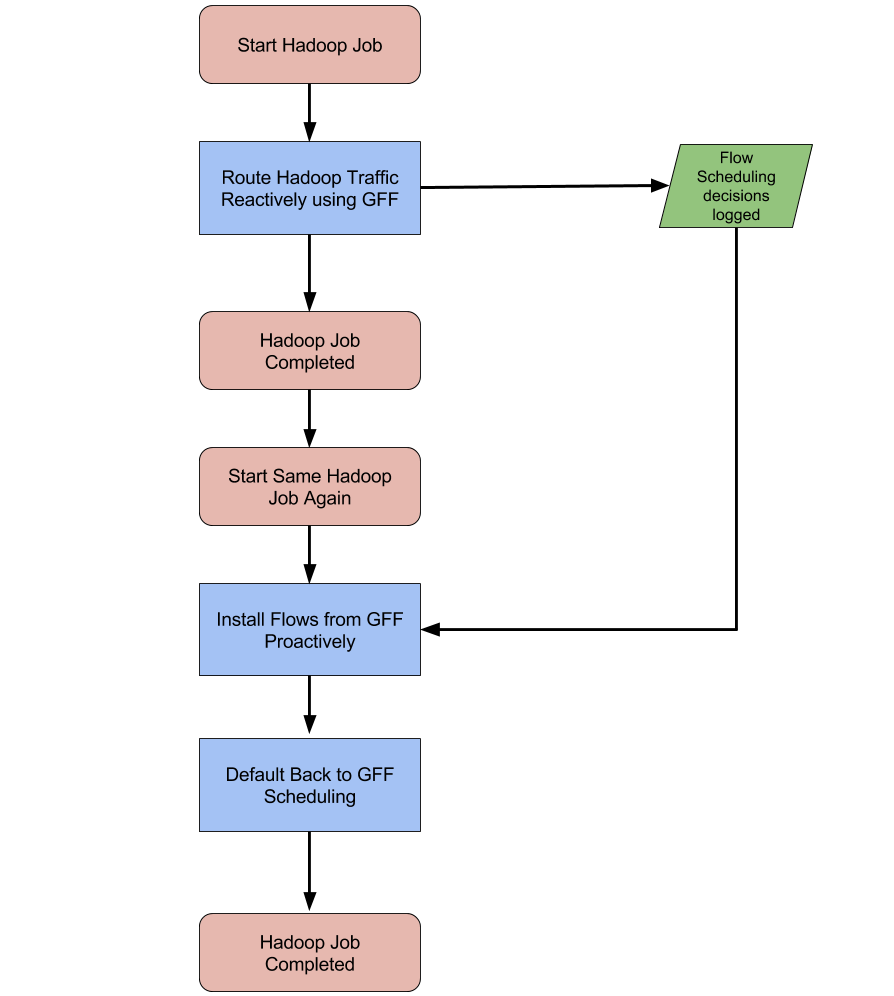
\includegraphics[scale=0.42]{graphics/chapter4/ProactiveAlgorithm.png}}
	\caption{A flowchart depicting the \textit{Proactive} Flow Scheduling Algorithm.}
	\label{fig:ProactiveAlgo}
\end{figure}
We device a proactive routing strategy as depicted in Figure \ref{fig:ProactiveAlgo} in the following steps
\begin{itemize}
	\item We run a Hadoop job on a cluster of 16 hosts, arranged in a \textit{fat-tree} \cite{al2008scalable} topology; where all switches in the network are controlled by a centralized controller using the OpenFlow \cite{mckeown2008openflow} protocol.
	\item Hadoop traffic is routed in the network using the Global First-Fit (GFF) \cite{al2010hedera} flow scheduling algorithm.
	\item The flow scheduling decisions made by the GFF algorithm are logged and persisted into the memory of the controller. 
	\item Concurrently, the total bytes transmitted and received by each host in the cluster are logged into disk, which are used to calculate the total bisection bandwidth achieved by the hosts in the network. 
	\item Subsequently, the same Hadoop Job is run again and the traffic of the network is handled by the \textit{Proactive} controller.
	\item The \textit{Proactive} controller reads the flow scheduling decisions for the same job made by the GFF algorithm earlier, and installs them statically in the network, prior to the start of Hadoop transfers.
	\item After installing flow entries statistically, it defaults to the GFF behaviour for routing flows in the network.  
	\item While the Hadoop job is running, each host in the network logs the total number of bytes transmitted and received by its network interface in order to calculate the average bisection bandwidth achieved for \textit{proactive} routing.
	\item The steps above are repeated iteratively for different Hadoop jobs. When all the iterations are completed, we obtain Hadoop Job completion times and  total bisection bandwidth utilization for our \textit{proactive} and GFF (\textit{reactive}) routing strategies.   
\end{itemize}

\section{Architecture Overview} \label{sec:DOverview}
The High-level architectural design of our experiment is illustrated in Figure \ref{fig:DesignOverview}, and it broadly consists of three parts: an SDN controller, a fat-tree data centre topology and a Hadoop Emulator. A brief overview of each part is provided in this section.
 
\begin{figure}[!ht] 
\centerline{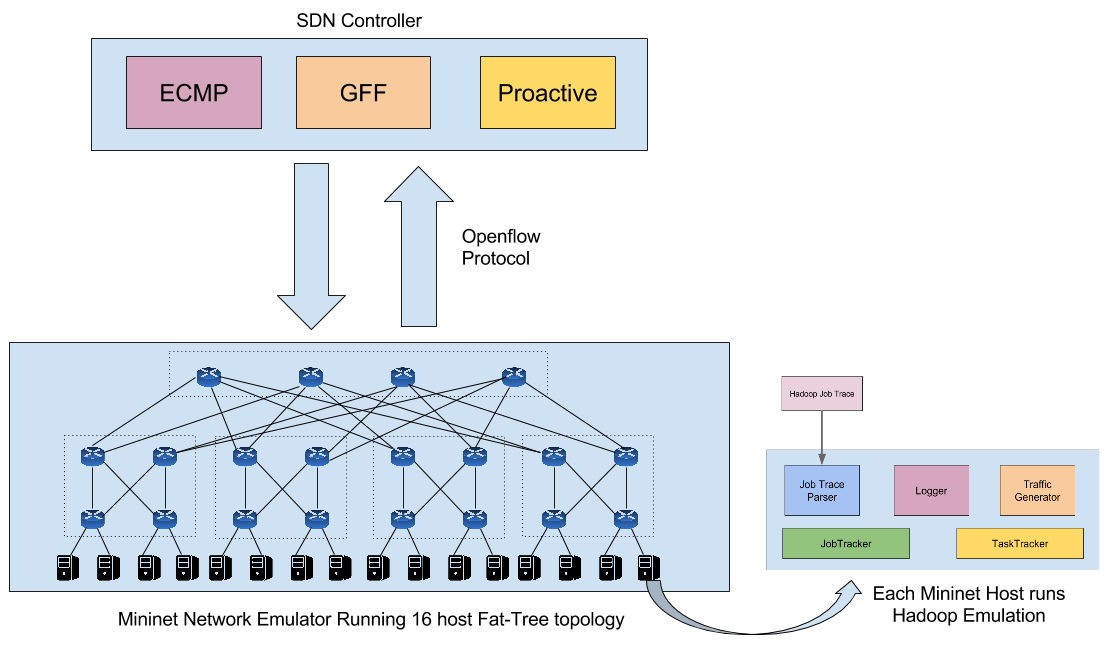
\includegraphics[scale=0.42]{graphics/chapter4/DesignOverview.png}}
\caption{High Level Overview of the experiment Design.}
\label{fig:DesignOverview}
\end{figure}

\subsection{SDN Controller}
The SDN controller has a three-fold functionality as illustrated in Figure \ref{fig:DesignOverview}. It routes Hadoop application traffic with three different routing algorithms, namely, ECMP \cite{hopps2000analysis} which is the \textit{de-facto} standard of routing traffic in a multi-rooted tree architecture \cite{al2008scalable}, Global First-Fit \cite{al2010hedera}, which is a \textit{reactive} flow scheduling algorithm that builds upon ECMP, and finally, our \textit{proactive} flow scheduling algorithm which leverages the \textit{reactive} flow decisions made by GFF for a certain Hadoop job, installing them statically before communication commences in the network for the same Hadoop job. 

At a time, it schedules flows using one of the three algorithms, which is specified when the SDN controller is launched. It controls the forwarding behaviour of all the switches in the fat-tree topology using the OpenFlow \cite{mckeown2008openflow} protocol as illustrated in Figure \ref{fig:DesignOverview}. 

\subsection{Fat-tree topology}

As mentioned in \ref{subsec:DataCentreEmulation}, we employ \textit{Mininet} \cite{lantz2010network} for emulating a data centre network, since we do not have access to a 16 host cluster. Therefore, we use the \textit{Mininet} network emulator for emulating a \textit{k}-ary fat-tree topology (described in \ref{subsec:Fat-Tree Topology}), where \textit{k} = 4 as illustrated in Figure \ref{fig:DesignOverview}. All the switches in the emulation are connected to an external SDN controller via the OpenFlow protocol, while each of the 16 hosts in the \textit{Mininet} emulator run a Hadoop emulation.

\subsection{Hadoop Emulation}

As illustrated in Figure \ref{fig:DesignOverview}, each host in the \textit{Mininet} emulator is running a Hadoop emulation. Since, the entire fat-tree topology is run on a single machine, it is not feasible to run a full version of Hadoop \cite{HadoopWeb} on the emulated hosts. Therefore, we use a lightweight alternative, by running a Hadoop emulator MRemu, on each host. As described in \ref{subsec:Mremu}, MRemu emulates Hadoop by producing iperf flows which are based on real Hadoop Job traces. Thus, we are able to simulate the running of Hadoop jobs in a 16 host fat-tree topology, where the routing decisions of the switches are controlled by an external SDN controller.   

\section{Analysis} \label{sec:DesignAnalysis}

Our aim in proposing the design of this \textit{Proactive} flow scheduling algorithm was to investigate if there are benefits in terms of better application performance and high bisection bandwidth utilization by \textit{proactive} configuration of a data centre network. 

In order to fulfil our aim, we introduced the design of our experiment in this chapter whereby we use \textit{reactive} configurations logged from the GFF algorithm, which are fed into the \textit{proactive} controller to be installed into the network as static flows. Automatic generation of proactive configuration for the network is beyond the scope of this project.

We find that the design set forth meets the requirements of this project, and is general enough to be applied to any Big data processing application traffic. It is a first step towards evaluating a \textit{proactive} measure of network configuration for big data application processing, owing to which it is straightforward to implement. The next chapter describes a proof-of-concept implementation of this design in python. 
  \chapter{Implementation} \label{chap:Implmentation}

The previous chapter described our proposed \textit{Proactive} flow scheduling algorithm and the design of our experiment. We leverage pre-existing \textit{reactive} flow scheduling decisions in the design of our \textit{Proactive} scheduler. In this chapter, we describe the implementation of our experiment design that has been employed to evaluate the effectiveness of our proposed \textit{Proactive} flow scheduler. In Section \ref{sec:ImplDesc}, an overall description of our design implementation is provided, outlining the working of different major components. In Section \ref{sec:ControlImpl}, the implementations of ECMP, GFF and our \textit{Proactive} flow scheduling SDN controllers are described. Moreover, Section \ref{sec:HadoopEmuImplementation} describes the structure of Hadoop job traces and functional working of the Hadoop emulation. In Section \ref{sec:ThroughputMeasure}, our implementation for measuring throughput from the hosts in the Hadoop emulation is described, and finally, Section \ref{sec:ImplSummary} summarises our design implementation.   


\section{Implementation description} \label{sec:ImplDesc}

We have implemented our \textit{Proactive} flow scheduling algorithm using the \textit{dart} branch \cite{POXdart} of the POX \cite{POXSDN} SDN controller. POX provides an extensible API written in Python, which can be used to program its controlling behaviour. As described in \ref{sec:Emulators}, we use the \textit{Mininet} Network Emulator \cite{lantz2010network} for emulating a 16 host fat-tree data centre topology, where each host is running a Hadoop emulation using \textit{MRemu} \cite{neves2015mremu}. The forwarding behaviour of the switches in the fat-tree network topology is controlled by the POX controller using OpenFlow \cite{mckeown2008openflow}. We run Hadoop jobs and measure Hadoop job completion times along with the total network bandwidth utilization for three flow scheduling algorithms, namely, ECMP \cite{hopps2000analysis}, Global First-Fit \cite{al2010hedera} and our \textit{Proactive} flow scheduling.

Figure \ref{fig:ExecutionOverview} illustrates the working of \textit{LaunchExperiment}, which is the main Python script that initiates the experiment. It builds a \textit{Mininet Network topology object}, by using a script from \textit{Ripl-POX} \cite{riplPOX} to initialize the switch, host and link configurations for a fat-tree network topology. \textit{Ripl-POX} is an extension to the POX controller which provides ECMP hash based routing, as described in \ref{subsec:ECMP}, and Mininet network configurations for data centre topologies such as \textit{fat-tree}, described in \ref{subsec:Fat-Tree Topology}.   

\begin{figure}[!ht] 
	\centerline{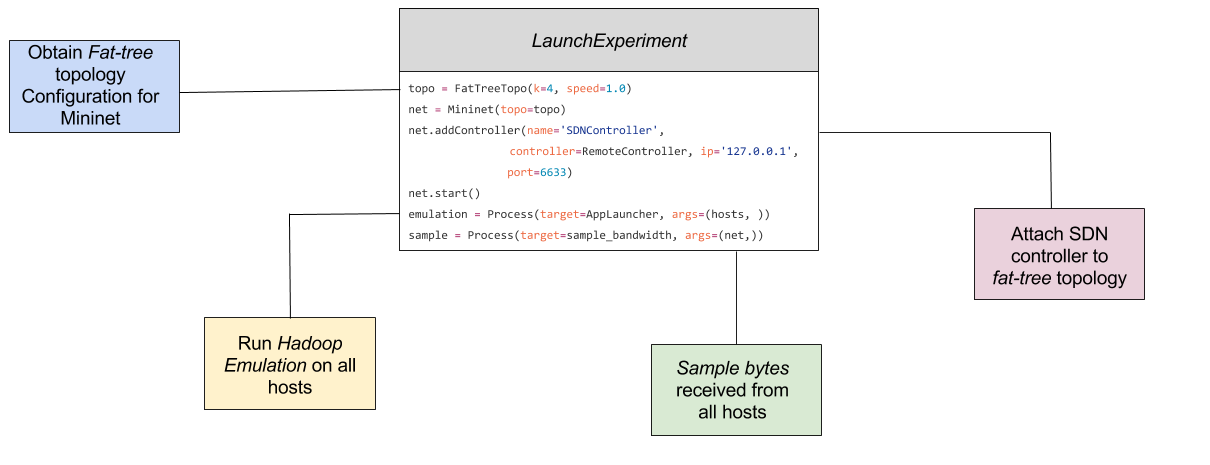
\includegraphics[scale=0.38]{graphics/chapter5/MainExecution.png}}
	\caption{Execution of the main script that loads the different modules of the experiment.}
	\label{fig:ExecutionOverview}
\end{figure}

Subsequently, a remote SDN controller is added to the Mininet network topology object by providing its IP address and port, as illustrated in the Figure \ref{fig:ExecutionOverview}, and the Mininet network emulation is launched. Finally, using Python's Multiprocessing library, two processes are launched simultaneously on each of the 16 hosts, where one of the process runs the Hadoop emulation as described in detail in Section \ref{sec:HadoopEmuImplementation}, while the second process samples the bytes received by the host from its network interface, described in detail in Section \ref{sec:ThroughputMeasure}.

\textit{LaunchExperiment} script illustrated in the Figure \ref{fig:ExecutionOverview} runs the experiment to measure \textit{total bisection bandwidth} achieved and \textit{Hadoop job completion times} when using different SDN remote controllers running on the IP address 127.0.0.1:6633, which are used for evaluating the effectiveness of our \textit{Proactive} flow scheduling against \textit{reactive} scheduling.      


\section{SDN Controller Implementation} \label{sec:ControlImpl}

In this section, we describe the Python-based implementation of our \textit{Proactive} controller along with implementations of ECMP and GFF controllers using the Python API of the POX SDN controller.

\subsection{Equal Cost Multi-Path Routing Implementation} \label{subsec:ECMPImpl}

As mentioned in \ref{sec:ImplDesc}, we used the ECMP routing implementation from \textit{Ripl-POX}, which is an extension of the POX controller.  ECMP routing is described in detail in \ref{subsec:ECMP}. It is the \textit{de-facto} industry standard routing mechanism for multi-path topologies \cite{al2010hedera} described in \ref{sec: DataCentreArch}, and attempts to spread traffic evenly in a network with multiple equal cost paths by hashing selected fields of an incoming packet modulo the total number of paths available and forwarding the packet along the path that corresponds to the result. 

\subsection{Global First-Fit Flow Scheduling Implementation} \label{subsec:GFFImpl}

Global First-Fit flow scheduling is an extension to ECMP routing for scheduling traffic in a topology with multiple equal cost paths between any two source and destination pairs of hosts, described in further detail in \ref{subsec:Hedera}. It maintains link capacities of all paths in the network. When a flow needs to be scheduled, GFF performs a linear search of all possible paths that can accommodate the flow, and allocates the first path that it encounters, which meets the bandwidth demands of the flow.   

The GFF controller class implementation \cite{gffImplementation} used in the experiment is illustrated in Figure \ref{fig:GFFClass}. Once all the switches in the fat-tree topology are connected to the GFF controller, the \textit{\_handle\_ConnectionUp}(event) function stores the switches in a Python list with the switch Data Path IDs which uniquely identify OpenFlow switches, as keys.  

\begin{figure}[!ht] 
	\centerline{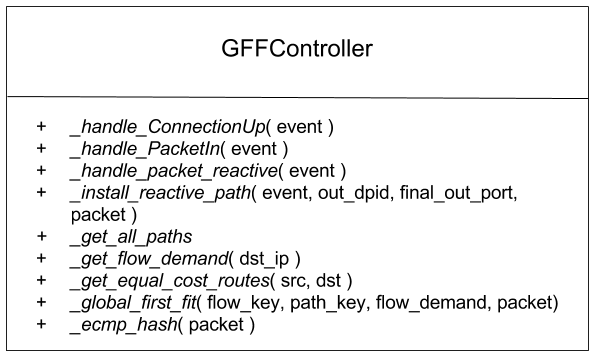
\includegraphics[scale=0.42]{graphics/chapter5/GFFClass.png}}
	\caption{Global First-Fit Network Controller Class}
	\label{fig:GFFClass}
\end{figure}

Subsequently, the \textit{\_get\_all\_paths}() function calculates equal cost routes by calling the \textit{\_get\_equal\_cost\_routes}(src, dst) function for all possible pairs of source and destination nodes in the network. When an OpenFlow switch gets a packet which has no matches in its forwarding table, the packet is sent to the SDN controller for processing \cite{mckeown2008openflow}. This event is handled by the \textit{\_handle\_packet\_reactive}(event) function, which responds by installing a flow entry in the switch, matching the header fields of the packet \textit{reactively}, using the GFF flow scheduling algorithm, and logs the header match fields along with the egress port into a JSON file, to be used later by the \textit{Proactive} controller. 

\subsection{Proactive Controller}

We implemented the \textit{Proactive} Controller on the \textit{hypothesis} that installing flows based on application traffic patterns in a proactive manner will reduce control overhead and high-level latencies caused due to installing of flows \textit{reactively}. Towards this end, we log flow scheduling decisions made by the GFF controller in a JSON file as described in \ref{subsec:GFFImpl}, for a particular Hadoop job. 
\begin{figure}[!ht] 
	\centerline{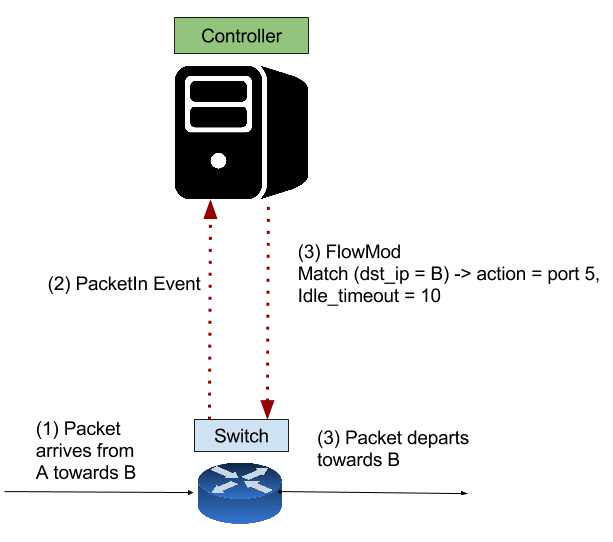
\includegraphics[scale=0.42]{graphics/chapter5/packetinOpenFlow.png}}
	\caption{Handling of \textit{packetIn} event on forwarding table miss by SDN controller using OpenFlow.}
	\label{fig:packetinOpenFlow}
\end{figure}
The same Hadoop job is run again and the logged flows from the previous execution are subsequently fed into the \textit{Proactive} controller, which installs them as soon as all the switches in the network are connected to it. Finally, for every \textit{packetIn} event \textit{i.e.}, when a packet is sent to the controller by a switch since its header fields do not match any entry in the switch's forwarding table as illustrated in Figure \ref{fig:packetinOpenFlow}, the controller procecsses the packet, and based on the control logic running in the controller, it creates \textit{FlowMod} message, with an action specifying the egress port of all packets matching  specific header fields. Subsequently, all packets matching the field as specified in the \textit{FlowMod} message are routed to same egress port by the switch till the entry times out. Similarly, after all the \textit{Proactive} entries time out, the proactive controller behaves like the GFF controller, by routing the packets \textit{reactively} on \textit{packetIn} events. 

Figure \ref{fig:ProactiveClass} illustrates the implementation of the \textit{Proactive} controller class using POX controller's Python API. Similar to the GFF controller class described in \ref{subsec:GFFImpl}, the \textit{\_handle\_ConnectionUp}(event) function stores all switches of the network connected to the controller corresponding to their data path IDs, in a Python list. Additionally, it calls the \textit{\_install\_proactive\_path}() function. 
\begin{figure}[!ht] 
	\centerline{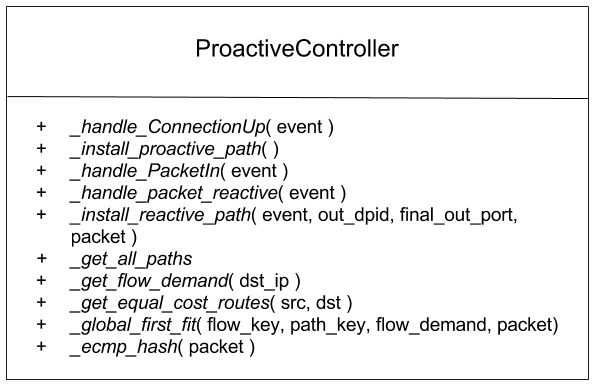
\includegraphics[scale=0.42]{graphics/chapter5/ProactiveClass.png}}
	\caption{Proactive Network Controller Class}
	\label{fig:ProactiveClass}
\end{figure}

The \textit{\_install\_proactive\_path}() function reads all the flow scheduling decisions made by the GFF controller, and installs the same in the appropriate switches. One of the sample flow scheduling decision logged by the GFF controller is illustrated in Figure \ref{fig:FlowRule}.

\begin{figure}[!ht]
\begin{lstlisting}[style=json]
{   
	"dl_type": 2048, 
	"nw_dst": "10.0.0.2", 
	"tp_dst": 6666, 
	"dpid": 1, 
	"tp_src": 48383, 
	"dl_dst": "00:00:00:00:00:02", 
	"dl_vlan": 65535, 
	"nw_src": "10.0.0.3", 
	"dl_src": "00:00:00:00:00:03", 
	"out_port": 2
}
\end{lstlisting}
\caption{Example of a flow decision obtained from GFF flow scheduler which is installed by the \textit{Proactive} network controller.}
\label{fig:FlowRule}
\end{figure}

Notable fields in the log of a flow scheduling decision include \textit{nw\_src}, \textit{nw\_dst}, \textit{dl\_src}, \textit{dl\_dst}, \textit{dpid} and \textit{out\_port} which are the source IP address, destination IP address, source Ethernet address, destination Ethernet address, switch data path ID and the output port respectively. All such logged flow decisions are installed by the \textit{Proactive} controller in the switches along with an \textit{IDLE\_TIMEOUT}, so that switch routing tables are not overwhelmed. Once the flow entries expire, traffic is routed in a \textit{reactive} manner, as described in \ref{subsec:GFFImpl}.   


\section{Hadoop Emulation Implementation} \label{sec:HadoopEmuImplementation}

Since it is not feasible to run a full version of Hadoop on emulated hosts, running on a single machine, due to memory and I/O constraints; therefore, we use a Hadoop emulator MRemu \cite{neves2015mremu}, as discussed in detail in \ref{subsec:Mremu}. It uses traces of real Hadoop Jobs to emulate Hadoop traffic patterns in an emulation running on a single machine, without the need of a real Hadoop cluster. In this section, we describe the structure of Hadoop application traces used in the experiment, and  briefly discuss the functional workflow of the Hadoop emulation.

\subsection{Hadoop Job Traces}

The Hadoop emulator generates traffic patterns in the network on the basis of Hadoop job traces, as discussed in detail in \ref{subsec:Mremu}. The MapReduce applications used to obtain these traces are discussed at length in \ref{sec:BenchTraces}. Information available in the Hadoop job traces is stored in JSON format. Figure \ref{fig:TraceExample} illustrates one element each from the \textit{transfers} and \textit{tasks} JSON arrays in a Hadoop trace. The elements of the \textit{transfer} array provide information about the network transfers and their durations, between two hosts. 

This information is used to generate \textit{iperf} flows between the source and destination hosts for the intended time duration, thereby simulating transfers of the real Hadoop job. 
Similarly, the \textit{task} array provides information pertaining to the different tasks assigned to the hosts in the network and their durations, which are simulated by the corresponding hosts.    

\begin{figure} [!ht]
\begin{lstlisting}[style=json]
{
	"transfers": [{
		"dstAddress": "172.27.102.16",
		"dstPort": 59861,
		"duration": 2.140714136,
		"finishTime": 1388441782.972,
		"mapper": "attempt_201312301708_0016_m_000014_0",
		"reducer": "attempt_201312301708_0016_r_000003_0",
		"size": 62584054,
		"srcAddress": "172.27.102.1",
		"srcPort": 50060,
		"startTime": 1388441780.831286
	}],
	"tasks": [{
		"finishTime": 1388441795.897,
		"host": "172.27.102.1",
		"name": "attempt_201312301708_0016_r_000002_0",
		"processingTime": 6.937,
		"shuffleFinished": 1388441788.953,
		"sortFinished": 1388441788.96,
		"sortingTime": 0.007,
		"startTime": 1388441772.748,
		"type": "REDUCE",
		"waitFinished": 1388441778.417361,
		"waitingTime": 5.669361
	}]
}
\end{lstlisting}
\caption{Example of a Hadoop job trace showing one element each from the transfers
	and tasks JSON arrays.} 
\label{fig:TraceExample}
\end{figure}


\subsection{Functional Architecture}

\textit{LoadExperiment} script executes the Hadoop emulation on all hosts in the network by launching the \textit{AppLauncher} class, as illustrated in Figure \ref{fig:ExecutionOverview}. Functional working of the Hadoop emulation on each host in the network is illustrated in Figure \ref{fig:HadoopEmuArch}. The \textit{AppLauncher} class executes Hadoop emulation on each host by obtaining information about the type of host, \textit{i. e.} if the host is the JobTracker or one of the TaskTrackers from the \textit{TraceParser} class. If the host's IP address corresponds to the JobTracker IP address in the Hadoop trace file, then it assumes the role of the JobTracker \textit{i. e.} the master node in the network, while all other hosts in the network assume the role of TaskTrackers.

\begin{figure}[!ht] 
	\centerline{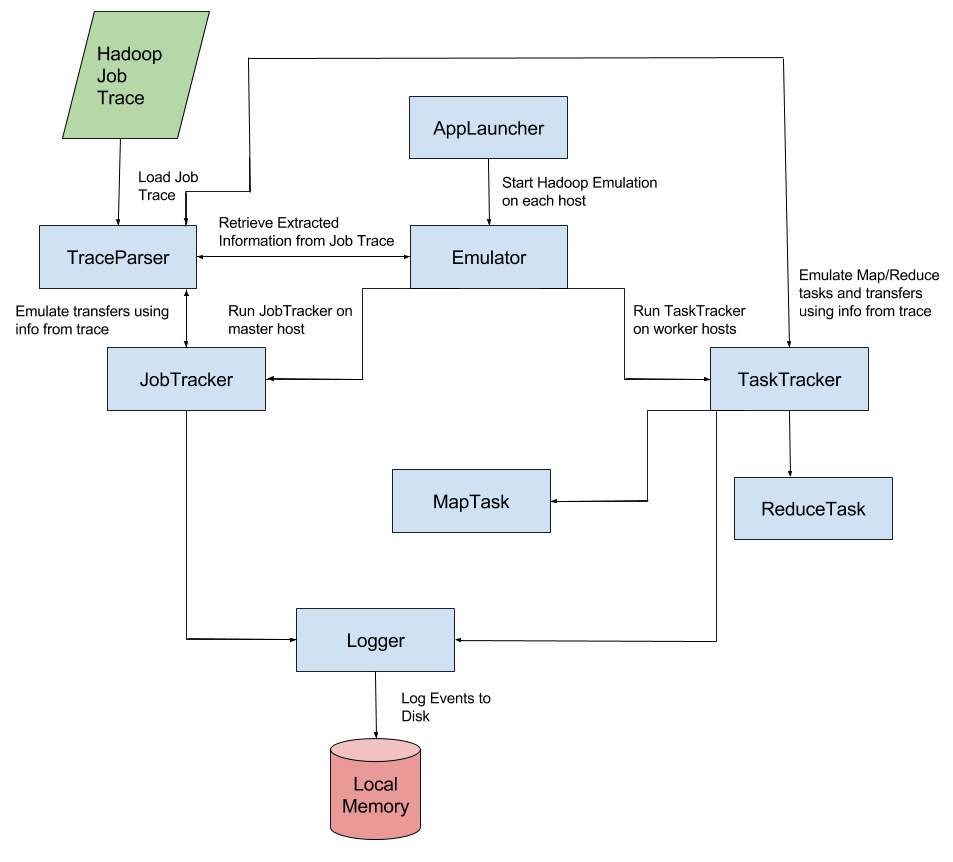
\includegraphics[scale=0.46]{graphics/chapter5/HadoopEmulationArchitecture.png}}
	\caption{Functional Architecture of the Hadoop Emulation.}
	\label{fig:HadoopEmuArch}
\end{figure}

TaskTrackers simulate the working of a Hadoop job by creating \textit{iperf} flows with the same durations as the actual transfer times, which are obtained from the \textit{TraceParser} class. Realistic latencies caused while running \text{Map/Reduce} tasks in Hadoop are also emulated by the TaskTrackers. Similarly, information about  the network traffic generated by the actual JobTracker is used to generate \textit{iperf} flows by the emulated JobTracker. Debug information from the emulated JobTracker and TaskTrackers about network events are logged in disk.      

\section{Throughput Measurement Methodology} \label{sec:ThroughputMeasure}

In this section, the implementation for sampling throughput in the emulated network of our experiment is discussed. In order to measure the total bytes received by a host in the network, we leverage information obtained from \textit{/proc/net/dev} directory of each host in the network.  

The \textit{/proc/} is a virtual Linux filesystem which is made available to user processes by the Linux kernel in order to share internal information about the system \cite{proc}. The \textit{/proc/net/} directory contains a number of files providing some aspect of information on networking of the Linux system. The contents of the files in the \textit{/proc/net/} directory can be viewed by using the \textit{cat} command. One such file in the \textit{/proc/net/} directory is the \textit{/proc/net/dev} file which provides information about the number of bytes transferred and received by the configured network interfaces of the system.      
\begin{figure}[!ht] 
	\centerline{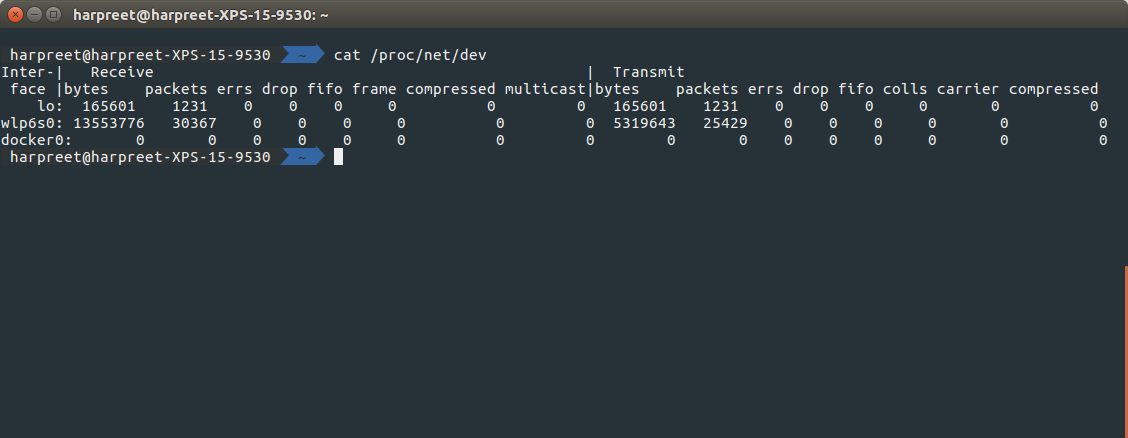
\includegraphics[scale=0.35]{graphics/chapter5/SamplingExample.png}}
	\caption{Sample output of \textit{cat /proc/net/dev} command.}
	\label{fig:ThroughputSamplingEg}
\end{figure}

A sample output of the \textit{cat /proc/net/dev} command is illustrated in Figure \ref{fig:ThroughputSamplingEg}. At any instant, it gives the total number of bytes transmitted and received by the configured network interfaces. This information is leveraged to calculate the total bisection bandwidth achieved by the emulated Hadoop traffic in the network, when routed via \textit{reactive} and \textit{proactive} approaches. 

Once the Hadoop emulation is executed on each host by the \textit{LaunchExperiment} script, it launches the \textit{sample\_bandwidth(net)} function simultaneously, as illustrated in \ref{fig:ExecutionOverview}, which measures the bandwidth used by each host in the network from the \textit{/proc/net/dev} file.

\begin{figure}[!ht] 
	\centerline{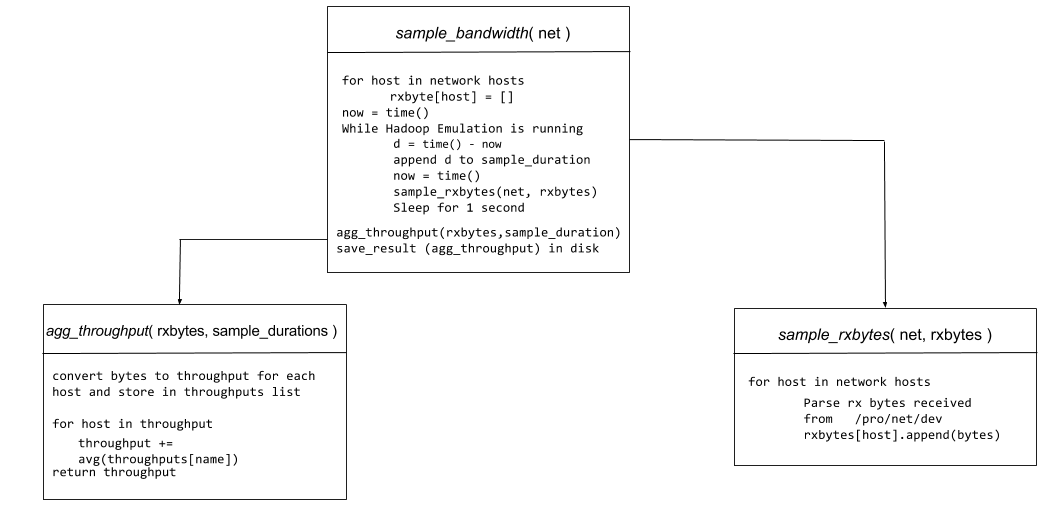
\includegraphics[scale=0.40]{graphics/chapter5/SamplingPseudocode.png}}
	\caption{Pseudocode for sampling of network throughput from all hosts in the network.}
	\label{fig:SamplingPseudocode}
\end{figure}

Pseudocode for sampling bandwidth utilized by each host is illustrated in Figure \ref{fig:SamplingPseudocode}. The \textit{sample\_bandwidth}(net) function creates an empty list of lists with the host objects as keys. Subsequently, while the Hadoop Emulation is running, it captures the total bytes received by the host interface by calling the \textit{sample\_rxbytes}(net, rxbytes) function, and storing the time duration between every two samples in a list. The \textit{sample\_rxbytes}(net, rxbytes) function captures the number of bytes received by the network interface by reading the contents of the \textit{/proc/dev/net} file and stores it in a list corresponding to the host object. 

When the Hadoop emulation terminates, the process of sampling bytes is stopped and the \textit{sample\_bandwidth}(net) function calculates the aggregate throughput achieved by calling the \textit{agg\_throughput}(rxbytes, sample\_durations), where the list of bytes sampled and the the durations of their sampling are sent as parameters. The \textit{agg\_throughput}(rxbytes, sample\_durations) function calculates the total aggregate throughput achieved by all the hosts in the network by converting the bytes to throughputs for each host and subsequently summing the average throughput achieved by each host in the network. 

\section{Summary} \label{sec:ImplSummary}

In summary, we implement the following components based on the design in Chapter \ref{chap:design}
\begin{itemize}
	\item An extension to the Global First-Fit flow scheduling controller which logs its flow scheduling decisions in a JSON file.
	\item A \textit{Proactive} controller that leverages the flow scheduling decisions logged by the Global First-Fit controller, by installing them \textit{proactively} and subsequently defaulting back to the \textit{reactive} behaviour of GFF controller.
	\item A mechanism to sample bytes received by each host in the network via the \textit{/proc/net/dev} directory, which is used to calculate the total throughput achieved by the hosts in the network.   
\end{itemize}


The next chapter discusses the tests carried out to  evaluate our implementation of the \textit{Proactive} flow scheduling mechanism by comparing it against the total throughput achieved by \textit{reactive} routing techniques and the effect of different flow scheduling mechanisms on Hadoop job completion times. 
   
  \chapter{Evaluation} \label{chap:eval}

The previous chapter detailed the implementation of our design proposed in Chapter \ref{chap:design}, including the implementation of our \textit{Proactive} flow scheduler. This chapter describes the benchmarking tests that were carried out to evaluate our \textit{Proactive} flow scheduler against ECMP and Global First-Fit flow scheduling algorithms. Section \ref{sec:ExperiSetup} describes our experimental setup. Subsequently, in Section \ref{sec:BenchTraces}, we describe the nature of Hadoop job traces used for evaluation. Section \ref{sec:EvalOverview} gives a brief overview of the methodology followed in obtaining experimental results. Sections \ref{sec:EvalBandwidth} and \ref{sec:EvalJobCompletion} provide a comprehensive description regarding the evaluation of total average bisection bandwidth achieved by the different flow scheduling mechanisms and their effect on Hadoop job completion times. Finally, in Section \ref{sec:CriticalAnalysisEval}, we summarize our findings and critically analyse the same. 


\section{Experimental Setup} \label{sec:ExperiSetup}

The tests described in this chapter were all run on a Dell Server with 8 x 3.40GHz cores of Intel Core i7-4770 processor, 16 GB of RAM, and 475.4 GB of hard disk space running Ubuntu 14.04 LTS operating system. The Python implementation of our experiment used Python version 2.7. The Hadoop traces used in our evaluation were obtained by Neves \textit{et al.} \cite{neves2015mremu} on a real cluster of 16 identical servers, each having 12 x86 64
cores, a single HDD and 128 GB of RAM, interconnected via 1 Gbps Ethernet links, running Hadoop 1.1.2 on top of Red Hat Enterprise Linux 6.2 operating system. 

For running our network emulations, we used the \textit{Mininet} network emulator from its cs244 branch version, since it is compatible with \textit{Ripl-POX} controller that is used for ECMP routing, as discussed in \ref{sec:ControlImpl}. For the Hadoop emulation, we used the MRemu emulator \cite{MRemuRepo2015}, and used POX \textit{dart} \cite{POXdart} SDN controller for flow scheduling of the emulated Hadoop traffic.

\section{Benchmark Traces} \label{sec:BenchTraces}

The Hadoop job traces used to generate traffic in our experiment were obtained from the MRemu github repository \cite{MRemuRepo2015}. The same traces were used by Neves \textit{et al.} \cite{neves2015mremu} to evaluate the performance of MRemu. The traces have been obtained from the following applications which are a subset of the HiBench benchmark suite \cite{huang2011hibench}
\begin{itemize}
	\item Sort - This application sorts text input data which is generated via a RandomTextWriter. Sort is used frequently to benchmark Hadoop performance. 32 GB of data was sorted to obtain Job traces.
	\item PageRank - It implements the page-rank \cite{huang2011hibench} algorithm which calculates web page ranks by taking the number of reference links in the web page as a metric. Hence, PageRank serves as a large-scale indexing application. Neves \textit{et al.} configured PageRank to process 500K pages, totalling approximately 1 GB of input size; and used the Pegasus Project \cite{kang2009pegasus} implementation of PageRank to obtain job traces.  
	\item Nutch - It is part of Apache Nutch \cite{NutchWeb}, which is a scalable and flexible web crawler that uses the MapReduce model for indexing pages in  large-scale web search engines. Nutch was configured to index 5M pages, which totalled to approximately 8GB of input data.
	\item Bayesian Classification - Another canonical use of MapReduce is large scale machine learning. This application uses a classification algorithm for data mining and knowledge discovery called Naive Bayesian \cite{huang2011hibench}. It forms a part of Apache Mahout, which is a popular machine learning library. To obtain Hadoop job traces, 100K pages were configured to be processed by Bayesian Classification.
\end{itemize}

However, the Hadoop job traces in the MRemu github repository \cite{MRemuRepo2015} have not been classified according to the Hadoop applications that were run in the real cluster setup to obtain them. Therefore, in our evaluation of the effect of different flow scheduling mechanisms on total bisection bandwidth achieved and the respective Hadoop job completion times for different Hadoop job traces, we were not able to classify the different Hadoop traces on the basis of the HiBench applications that were used in order to obtain them. This is a limitation in our evaluation of the different routing mechanisms since different traces have achieved different levels of the network bisection bandwidth and we were not able to explore the causes for the same.    

\section{Evaluation Overview} \label{sec:EvalOverview}
We evaluated the effect of different routing mechanisms on the total bisection bandwidth achieved and Hadoop job completion times by running tests in the following manner

\begin{itemize}
	\item Firstly, we launched the POX controller with ECMP routing.
	\item While the ECMP controller was running, we launched the Mininet network emulation of a 16 host fat-tree topology with each host running the Hadoop emulation. 
	\item Subsequently, we stored the total bandwidth achieved and the total job completion times to disk, once the Hadoop emulation was over.
	\item We followed the same procedure listed above while running Global First Fit flow scheduling and our \textit{Proactive} flow scheduling in the POX controller instead of ECMP scheduling, and logged the total bandwidth achieved by the hosts in the emulation and their respective job completion times to disk.    
\end{itemize}

The above procedure was repeated for different Hadoop job traces and the results obtained are discussed in the following sections. 

\section{Evaluation of Total Bisection Bandwidth Achieved} \label{sec:EvalBandwidth}

After running benchmark tests as described in the previous section, we plotted the total throughput achieved for ECMP, GFF and \textit{Proactive} flow scheduling for different Hadoop job traces on the graph illustrated in Figure \ref{fig:RoutingVThroughput}. Global First-Fit flow scheduling was observed to outperform ECMP routing in all instances, achieving \textbf{24.21}\% more throughput on average than ECMP routing.  

 
\begin{figure}[!ht]
	\centerline{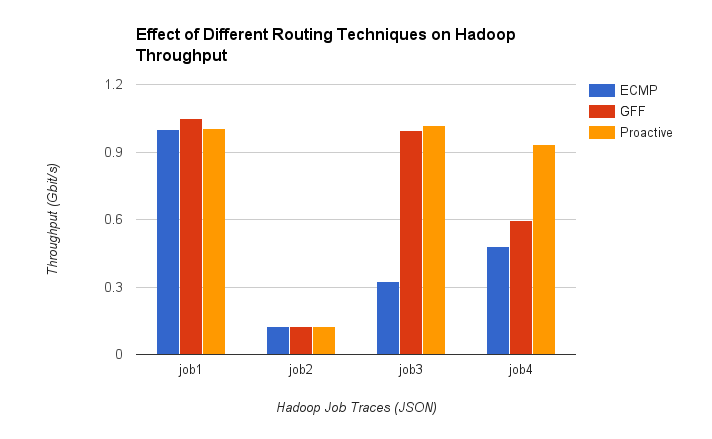
\includegraphics[scale=0.66]{graphics/chapter6/RoutingVThroughput.png}}
	\caption{Total throughput achieved by hosts running Hadoop job emulation in an emulated network with 1 Gbps links, grouped by the throughput achieved when running different Hadoop jobs for ECMP routing, Global First-Fit flow scheduling and \textit{Proactive} flow scheduling. On average, \textit{Proactive} flow scheduling was found to achieve \textbf{59.9}\% more bandwidth than ECMP routing and \textbf{11.6}\% more bandwidth than GFF flow scheduling.}
	\label{fig:RoutingVThroughput}
\end{figure}

Al-Fares \textit{et al.} \cite{al2010hedera} found Global First-Fit to outperform ECMP by achieving \textit{39}\% more of the total bisection bandwidth available in the network. The difference of \textit{15}\%, between our results and the ones obtained by Al-Fares \textit{et al.} might be attributed to the fact that we run our experiment on a single server, causing the GFF flow scheduler to perform slower due to limited computational resources. 

Our \textit{Proactive} flow scheduling mechanism was observed to perform significantly better than ECMP, achieving \textbf{59.9}\% more of the total bisection bandwidth available in the network than ECMP routing. In comparison to Global First-Fit routing, the \textit{Proactive} flow scheduler was comparable for the first two of the Hadoop Job traces, \textit{i. e.} \textbf{job1} and \textbf{job2} respectively, while for \textbf{job3} and \textbf{job4}, \textit{Proactive} flow scheduling outperformed Global First-Fit scheduling, as illustrated in Figure \ref{fig:RoutingVThroughput}. On an average, the \textit{Proactive} flow scheduler achieved \textbf{11.6}\% more of the total bisection bandwidth available in the network than Global First-Fit flow scheduling. 

Since we are not aware of the exact nature of the Hadoop job traces used in the evaluation of the \textit{Proactive} controller against ECMP routing and GFF flow scheduling, as described in \ref{sec:BenchTraces}, therefore, we cannot point out the reasons for \textit{Proactive} flow scheduling to outperform \textit{Global First-Fit} scheduling for \textbf{job3} and \textbf{job4} Hadoop traces respectively, while performing comparably to \textit{Global First-Fit} routing for \textbf{job1} and \textbf{job2} Hadoop traces, as illustrated in Figure \ref{fig:RoutingVThroughput}. Nonetheless, the results obtained substantiate our claim that \textit{Proactive} flow scheduling improves network performance by reducing the amount of control overhead in the network.      

The throughput readings used in Figure \ref{fig:RoutingVThroughput} were taken by re-running the tests described in \ref{sec:EvalOverview}, and taking the \textit{mode} of the throughput values obtained, so as to avoid \textit{Random Errors} in the values since the experiment was compute intensive. 

\section{Evaluation of Hadoop Job Completion Times} \label{sec:EvalJobCompletion}

As described in \ref{sec:EvalOverview}, we observed the Hadoop job completion times when traffic was routed following ECMP, Global First-Fit and \textit{Proactive} scheduling mechanisms respectively, for different Hadoop Job traces and plotted the readings on the graph illustrated in Figure \ref{fig:RoutingVJobCompletion}. We found the Hadoop job completion times to \textit{correlate} with the average bisection bandwidth achieved by hosts in the emulated network, when traffic was routed following the three flow scheduling algorithms, as described in the previous section.

\begin{figure}[!ht]
	\centerline{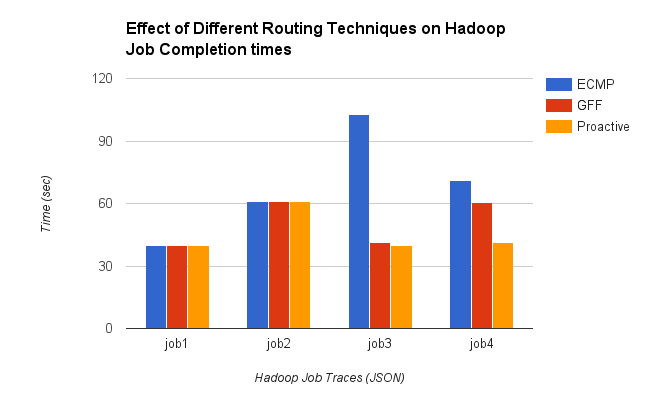
\includegraphics[scale=0.66]{graphics/chapter6/RoutingVJobCompletion.png}}
	\caption{Time taken to complete Hadoop job emulation by hosts in an emulated network with 1 Gbps links, grouped by Hadoop job completion times when running different Hadoop jobs for ECMP routing, Global First-Fit flow scheduling and \textit{Proactive} flow scheduling. \textit{Proactive} Flow scheduler achieves  lower Hadoop job completion times by \textbf{35.58}\% in comparison to ECMP routing and \textbf{10.07}\% in comparison to Global First-Fit flow scheduling.}
	\label{fig:RoutingVJobCompletion}
\end{figure}


\textit{Hadoop job completion times} were found to have an  \textbf{inverse correlation} with the \textit{total bisection bandwidth} achieved, indicating that flow scheduling mechanisms that achieve a higher bisection bandwidth result in lowering of Hadoop job completion times. We calculated Pearson product-moment correlation coefficient for average throughput achieved by different routing mechanisms as the dependent variable and the average time taken for Hadoop job completion by different routing mechanisms as the independent variable, and found the \textit{correlation coefficient} to be \textbf{-0.9981}, which is indicative of total negative correlation between the two. 

Moreover, Global First-Fit scheduling was found to lower Hadoop job completion times by \textbf{15.07}\% in comparison to ECMP scheduling, while the \textit{Proactive} Flow scheduler was found to lower Hadoop job completion times by \textbf{35.58}\% in comparison to ECMP scheduling and \textbf{10.07}\% in comparison to Global First-Fit flow scheduling. 

\section{Critical Analysis of Experiment Results} \label{sec:CriticalAnalysisEval}
As mentioned in Section \ref{sec:BenchTraces}, the Hadoop job traces used were a subset of the HiBench benchmark suite of MapReduce applications, specifically, Sort, Nutch, PageRank and Bayesian Classification, produced by Neves \textit{et al.} \cite{neves2015mremu}, made available on the MRemu github repository \cite{MRemuRepo2015}. However, they were not classified into their application types, hence we were not able to account for the reasons behind the difference in bisection bandwidth achieved by different Hadoop job traces as illustrated in Figure \ref{fig:RoutingVThroughput}; which is a limitation of our evaluation.  
\begin{figure}[!ht]
	\centerline{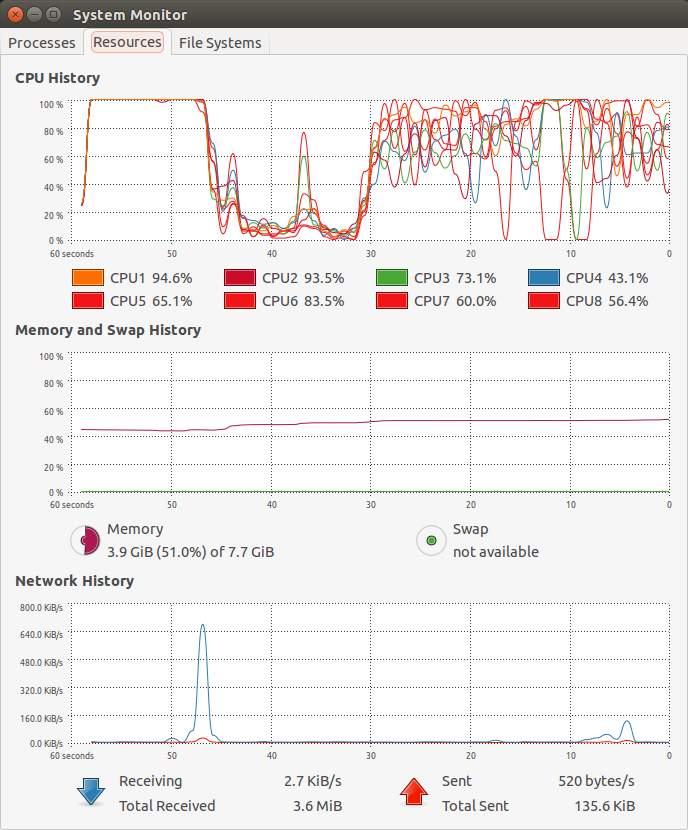
\includegraphics[scale=0.35]{graphics/chapter6/CPUUtilization.png}}
	\caption{A screenshot of the CPU utilization while the experiment was running on the server.}
	\label{fig:CPUutilization}
\end{figure}

Nonetheless, we were able to evaluate the bandwidth achieved and Hadoop job completion times for ECMP, GFF and our \textit{Proactive} flow scheduling mechanisms. Global First-Fit was found to achieve 24\% more aggregate bandwidth than ECMP. Al-Fares \textit{et al.} reported this difference to be 39\%. We speculate the difference in our findings to be attributed to the fact that our experimental setup involved a single server emulating 16 hosts arranged in a fat-tree topology, resulting in a  computation bottleneck as illustrated in Figure \ref{fig:CPUutilization}, which is a screenshot of the Ubuntu System Monitor utility, taken while the emulation was running, showing that at certain point of time, all 8 cores of our server used for the experiment were running at full processing utilization. 

We evaluated our \textit{Proactive} flow scheduling mechanism against ECMP and Global First-Fit flow scheduling, and observed an average gain of \textbf{59.9}\% and \textbf{11.6}\% in total bisection bandwidth achieved against ECMP and Global First-Fit flow scheduling respectively. Moreover, \textit{Proactive} flow scheduling achieved faster Hadoop job processing times by \textbf{35.58}\% and \textbf{10.07}\% in comparison to ECMP and Global First-Fit flow scheduling, highlighting the potential of \textit{Proactive} Network configuration approaches to optimize performance of Big Data applications. Moreover, we found the total bisection bandwidth and Hadoop job completion times to be negatively correlated by Pearson's correlation coefficient of \textbf{-0.99}, which underlines the huge potential of \textit{Reactive} and \textit{Proactive} Network configuration to enhance the performance of Big Data processing applications in a data centre network.
  \chapter{Conclusion} \label{chap:conc}

In the previous chapter, we summarized our evaluation of the \textit{Proactive} flow scheduler in terms of its  performance and compared it with ECMP routing and Global First-Fit flow scheduling. In this chapter, we will summarize the project and our results, and discuss possible future work.

\section{Project Overview}

Recent years have seen a steady growth in the amount of data generated by mobile and web applications, which is the fuel that drives Big Data Analytics. Mayer-Sch{\"o}nberger \textit{et al.} \cite{mayer2013big} define "big data" as the ability of harnessing information in novel ways thereby producing valuable insights or goods of significant value. As the data volumes grow, big data processing frameworks such as Hadoop \cite{HadoopWeb} require scaling out to thousands of commodity servers, subsequently resulting in an increase in the network traffic. Network performance has been found out to be of paramount importance for optimizing the processing times of Big Data applications, since research \cite{al2010hedera, greenberg2009vl2,guo2008dcell} has determined the network to be a performance bottleneck.

Recent studies \cite{al2008scalable, greenberg2009vl2, guo2008dcell,guo2009bcube} propose horizontal scaling of hosts to thousands of commodity servers in multi-rooted tree topologies, such as a \textit{fat-tree} topology that exploit path diversity to overcome limited port densities in commodity switches, thereby scaling the network with the increasing number of servers required to process large volumes of data. Moreover, emergent technologies such as Software-Defined Networking enable programming of the network stack, by maintaining a global view of the network state which is enabled by the separation of the control plane from the data plane of forwarding devices \cite{lantz2010network}. 

Various research efforts \cite{das2013transparent, wang2012programming, al2010hedera, narayan2012hadoop, neves2014pythia, wette2015hybridte} have tried to make the network dynamically reconfigure according to application traffic demands, in order to avoid congestion and optimize big data processing in a data centre network. Dynamic network reconfiguration approaches are \textit{reactive} in nature and try to optimize network performance by either being \textit{application-aware}, where the big data application controller reports traffic demands to the network controller which subsequently reconfigures the network accordingly, or by adopting the approach of \textit{traffic-awareness}, where a network monitor provides information to the network controller for \textit{reactive} reconfiguration. However, such \textit{reactive} measures of network configuration are bound to induce control traffic in the network and cause high level latencies in reconfiguring the network dynamically. 

We propose a \textit{Proactive} approach for the configuration of a data centre network, which installs flow rules in the network before the big data application starts. The flow rules are obtained from the previous execution of the same application when it is routed by the \textit{Global-First Fit} \cite{al2010hedera} flow scheduling algorithm, which is a \textit{traffic-aware} algorithm that builds upon \textit{Equal Cost Multi-Path} (ECMP) routing. ECMP is the standard routing protocol in multi-rooted data centre networks with path \textit{multiplicity}. Our \textit{Proactive} network controller reverts to Global First-Fit flow scheduling once the \textit{proactive} flows installed by it in the forwarding devices expire. 

In order to evaluate our \textit{Proactive} network controller against ECMP routing and Global First-Fit flow scheduling, we ran emulations of Hadoop jobs on a 16 host \textit{fat-tree} topology, running on a single server, and measured the effect of the different flow scheduling mechanisms on total bisection bandwidth achieved by the hosts in the network and Hadoop job completion times. An average gain of \textbf{59.9}\% and \textbf{11.6}\% in total bisection bandwidth achieved by the hosts in the network in comparison to ECMP routing and Global First-Fit flow scheduling was observed, when network traffic was routed by the \textit{Proactive} controller. Moreover, the \textit{Proactive} controller reduced Hadoop job completion times by \textbf{35.58}\% and \textbf{10.07}\% in comparison to ECMP routing and Global First-Fit flow scheduling. 

Automatic generation of \textit{Proactive} configurations for the network was beyond the scope of this project, therefore we used the network configurations generated by Global First-Fit flow scheduling. The results obtained by us indicate that \textit{proactively} configuring the network results in an increase in the total network utilization which benefits the performance of big data processing applications. Given that current \textit{application-aware} and \textit{traffic-aware} approaches of dynamic network configuration are not optimized with \textit{Proactive} configurations, there may be more to be gained in terms of average network bisection bandwidth utilization, if they are optimized before deployment.  

\section{Contribution}
In summary, our project validates the effectiveness of \textit{Proactive} configuration of data centre networks in optimizing big data application performance. Our evaluation results demonstrate that \textit{reactive} approaches have a lot to gain if they are optimized \textit{proactively} before deployment, since our \textit{Proactive} flow scheduler is able to achieve higher bisection bandwidth utilization in a data centre network and lower Hadoop job completion times than current static ECMP routing and \textit{reactive} approaches explored in research, such as Global First-Fit flow scheduling. 

Furthermore, we established a \textit{high negative correlation} between total bisection bandwidth achieved in the network and Hadoop job completion times, further highlighting the significance of network performance in accelerating big data applications.  

\section{Future Work}

While our \textit{Proactive} flow scheduling approach has increased the network performance in terms of the total bisection bandwidth achieved, it relies on flow scheduling decisions made by the \textit{Global First-Fit} algorithm for the same Hadoop job. In order to fully explore the effect of \textit{Proactive} configuration of the network, the network has to be configured proactively based on the application communication patterns. A future extension to our \textit{Proactive} flow scheduler might be to independently install \textit{Proactive} configurations in the network by generating them automatically, on the basis of application communication patterns.

We based our experiment on an emulation based testbed, since we did not have access to the hardware resources for deploying our implementation on a real cluster of 16 hosts. Moreover, for the same reason, we used the Hadoop job traces obtained by Neves \textit{et al.} \cite{neves2015mremu}, which were not classified according to the MapReduce applications that were run to obtain the traces, thereby hindering our ability to account for the difference in total bisection bandwidth achieved for different Hadoop job traces as discussed in Chapter \ref{chap:eval}. Consequently, a future extension to our experiment would be to obtain Hadoop job traces from a real cluster and subsequently run the experiment on the same, in order to validate the findings from our emulation based testbed and account for the difference in the average bisection bandwidth achieved for different Hadoop applications.   

\section{Final Remarks}

Big Data processing is being used to solve complex problems of society by levering enormous volumes of data available from ubiquitous computing devices. In order to ensure robust performance of big data applications, data centre networks have to be configured according to application communication patterns, so that traffic congestion in the network is avoided. By utilizing the emergent technology of Software-Defined Networking, the network stack can be programmed to configure a data centre network in accordance with application communication patterns, enabling scalability of network performance as more commodity servers are added into the network in order to deal with the growing data volumes. We showed that optimizing the network \textit{proactively} results in performance gains over current \textit{reactive} approaches and hope that as research evolves out in this field, the full potential of \textit{Proactive} network configuration for optimizing big data processing will be exploited.   


%\addcontentsline {toc}{chapter}{Appendices}       %% Force Appendices to appear in contents
\begin{appendix}
\chapter{Abbreviations}

\begin{tabular}{p{40mm}|p{100mm}}
	\textbf{Short Term}&\textbf{Expanded Term}\\
	\hline
	SDN&Software Defined Networking\\
	ECMP&Equal Cost Multi-Path\\
    RPC&Remote Procedure Call\\
	HDFS&Hadoop Distributed File System\\
    MR&MapReduce\\
    CPU&Central Processing Unit \\
    ToR&Top of Rack \\
    TCAM&Ternary Content Addressable Memory \\
    GFF&Global First Fit
\end{tabular}

\chapter{Source Disk Contents}

This document also includes a source disk containing:

\begin{itemize}
	\item The complete source code and referenced libraries for the Python implementation described in Chapter \ref{chap:Implmentation}, along with a readme file for running the experiment (in the folder \textbf{src}),
	\item A spreadsheet with the results obtained for evaluating the experiment in Chapter \ref{chap:eval} (in the folder \textbf{results}). 
\end{itemize}

\end{appendix}


%\addcontentsline {toc}{chapter}{Bibliography}     %% Force Bibliography to appear in contents

% \begin{thebibliography}{ieeetr}                   %% Start your bibliography here; you can
% %\bibliography{refs}                               %% also use the \bibliography command

% \input{biblio}
%\end{thebibliography}                             %% to generate your bibliography.

\bibliographystyle{plain}
\bibliography{references} 


\end{document}                                    %% END THE DOCUMENT
